\documentclass[a4j,10pt]{ujarticle}
\usepackage[schinese,japanese]{pxbabel}
\usepackage[dvipdfmx]{graphicx,color}
\usepackage{caption,subcaption}
\usepackage{amsmath,mathtools}
\usepackage{bm}
\usepackage{siunitx}
\usepackage{amssymb}
\usepackage{tikz}
\usepackage{xcolor}
\usepackage{tabularx}
\usepackage{array}
\usetikzlibrary{arrows.meta,matrix,calc,positioning,fit}

\usepackage[dvipdfmx,
            colorlinks,
            breaklinks,
            urlcolor = blue,
            linkcolor = black,
            citecolor = blue]{hyperref}  %放最后
\usepackage{cleveref}
    \crefname{section}{}{}
    \creflabelformat{section}{#2#1節#3}
    \crefname{figure}{}{}
    \creflabelformat{figure}{#2図#1#3}
    \crefname{table}{}{}
    \creflabelformat{table}{#2表#1#3}
    \crefname{equation}{}{}
    \creflabelformat{equation}{#2式(#1)#3}
    \crefname{appendix}{}{}
    \creflabelformat{appendix}{#2付録#1#3}
    \newcommand{\crefpairconjunction}{と}
    \newcommand{\crefrangeconjunction}{から}
\usepackage{pxjahyper} % hyperrefにおける目次の文字化け問題を調整


\begin{document}
% ============================================================
% Title
% ============================================================

\title{
実シーケンシングデータに対する量子アニーリングDNAアセンブリ\\
}

\author{陸永茂、肖一飛}
\date{}

\maketitle

\vspace{5mm}

% ============================================================
% Table of Contents
% ============================================================

\renewcommand{\contentsname}{目次}
\setcounter{tocdepth}{2}
\tableofcontents

\newpage
\section{はじめに}

DNA sequencing では、元の長い DNA 配列を一度に完全に読み取るのではなく、多数の短い断片として読み取る。この一つ一つの断片を read と呼び、read 間の重なり、すなわち overlap を手がかりとして正しい並びを推定し、元の DNA 配列を復元する問題が DNA assembly である。量子アニーリングを DNA assembly に利用する研究はすでに報告されている。例えば QuASeR \cite{sarkar2021quaser} では DNA assembly を QUBO として定式化し、D-Wave 2000Q 上で直接扱われた最大規模は 9 reads であった。また Boev et al.\ \cite{boev2021genome} は bacteriophage $\phi$X174 を対象として genome assembly を量子最適化問題として定式化しているが、計算には既知の reference genome から人工的に生成した 50 reads が用いられている。

このような人工データは、ハミルトニアンや量子アルゴリズムそのものを検証する上では有用である。しかし、実際の sequencing data には sequencing error、coverage の不均一性、repeat、曖昧な overlap などが含まれ、それらによってアセンブリグラフには分岐、合流、サイクルが現れる \cite{li2016miniasm,kamath2017hinge,kolmogorov2019flye}。そのため、小規模な人工データで正しい解が得られたとしても、同じ方法をそのまま実データへ拡張できるとは限らない。特に、read 数と候補 overlap 数が増加すると、グラフ全体を一つの QUBO に変換した場合に必要となる二値変数や二次結合の数も急速に増加する。一方で、アセンブリグラフのすべての部分が同じ計算難易度を持つわけではない。サイクルを含まない有向非巡回グラフ（DAG）であれば、最長経路は動的計画法によって古典的かつ厳密に求めることができる。本研究ではこの違いに着目し、グラフ全体を量子アニーリングで直接解くのではなく、古典計算で処理できる部分と、組合せ最適化を必要とする循環部分を分けて扱う。

実データに対してこの方針を実現するには、大規模なアセンブリグラフから古典計算で処理できる部分を切り分け、循環によって生じる曖昧性を十分小さな局所問題へ縮約する必要がある。そこで本研究では、DAG 部分を古典計算で厳密に処理しながらグラフを階層的に縮約するグラフ圧縮法を構成する。さらに、縮約後にも残る小さな循環部分に対して、始点--終点経路をサイクル問題として表現し、量子アニーリングで扱うためのハミルトニアンを導入する。本研究の目的は、単に従来より大きな QUBO を解くことではない。実シーケンシングデータから得られる大規模なアセンブリグラフをその構造に応じて古典計算と組合せ最適化に分担させ、必要な部分だけを量子アニーリングへ渡し、得られた局所解から最終的に元の read path を復元できる一連の処理方法を構築することである。

本報告では、まず第2章で DNA assembly と OLC グラフの基本的な問題設定を説明し、実データで分岐、合流、サイクルが生じる理由と、DAG と循環グラフの計算上の違いを整理する。第3章では、量子アニーリングによる DNA assembly の先行研究をもとに既存の QUBO 定式化を復現し、小規模問題に対するハミルトニアンの挙動を調べるとともに、それを大規模な実データへ拡張する際に生じる問題を検討する。第4章では、グラフ圧縮後にも残る小さな循環問題を量子アニーリングで扱うため、始点--終点経路をサイクル問題へ変換する方法と、辺の位置情報に基づく循環問題用ハミルトニアンを導入し、大きな固定ペナルティを避けるための大関法についても議論する。第5章では、本研究で構成したグラフ圧縮法について説明する。局所的な DAG 部分を動的計画法で厳密に処理し、循環部分をより小さな局所問題へ段階的に縮約する方法と、縮約後にも元の read path を復元するために必要な情報を保持する方法を示す。さらに、$\phi$X174、CHM13、\textit{C.~elegans}、\textit{Candida} の実シーケンシングデータを用いて、実際のアセンブリグラフがどの程度まで小さな問題へ縮約されるかを評価する。最後に第6章で、現在までに得られた結果を整理し、グラフ圧縮法、循環問題用ハミルトニアン、量子アニーリングを実シーケンシングデータから最終的な DNA 配列の再構成まで一つの処理系として接続するための今後の課題を述べる。








% ============================================================
\section{背景知識：DNA assembly と OLC グラフ}
% ============================================================

DNA assembly を計算問題として扱うには、read 同士の overlap がどのように元の配列の順序を決め、それがどのようなグラフ構造として現れるかを明確にする必要がある。単純な場合には read の接続順序はほぼ一意に決まるが、実シーケンシングデータでは分岐、合流、サイクルが生じる。以下では、この違いが OLC グラフ上の経路探索の計算量にどのように反映されるかを整理する。


% ============================================================
\subsection{read をつなげて元の DNA を復元する}
% ============================================================

DNA assembly では、異なる read に含まれる共通部分、すなわち overlap を手がかりとして read の並びを推定する。例えば、元の配列が
\[
\mathrm{ACGTACGTTAGC}
\]
であり、
\[
r_1=\mathrm{ACGTAC},\qquad
r_2=\mathrm{TACGTT},\qquad
r_3=\mathrm{GTTAGC}
\]
という三つの read が得られたとする。$r_1$ と $r_2$ は \texttt{TAC}、$r_2$ と $r_3$ は \texttt{GTT} を共有しているため、この例では
\[
r_1\rightarrow r_2\rightarrow r_3
\]
と並べることで元の配列を復元できる。図\ref{fig:assembly_simple}は、この最も単純な assembly の考え方を示している。

% ============================================================
% Figure 1
% ============================================================

\begin{figure}[tbp]
\centering
\begin{tikzpicture}[
  >=Latex,
  read/.style={
    draw,
    rounded corners=1.5mm,
    minimum width=25mm,
    minimum height=8mm,
    align=center,
    font=\small
  },
  ar/.style={->,thick},
  lab/.style={font=\scriptsize}
]

\node[read] (r1) at (-3.8,0)
{$r_1$\\\texttt{ACGTAC}};

\node[read] (r2) at (0,0)
{$r_2$\\\texttt{TACGTT}};

\node[read] (r3) at (3.8,0)
{$r_3$\\\texttt{GTTAGC}};

\draw[ar] (r1)
-- node[above,lab]{overlap} (r2);

\draw[ar] (r2)
-- node[above,lab]{overlap} (r3);

\node[font=\small] at (0,-1.15)
{read の overlap から接続順序を決める};

\end{tikzpicture}

\caption{
DNA assembly の最も単純な例。read 間の overlap を利用して元の DNA 配列を復元する。
}
\label{fig:assembly_simple}
\end{figure}

この例では接続候補が一意であるため、read の順序をそのまま決めることができる。実データでは一つの read に複数の接続候補が存在するため、read を一列に並べて考えるだけでは全体の接続関係を表しにくい。そこで、read 間の overlap をグラフとして表現する。


% ============================================================
\subsection{OLC グラフ}
% ============================================================

read を頂点、read 間の overlap 候補を有向辺として表すと、どの read からどの read へ接続できるかを一つのグラフとして記述できる。本研究では、この表現として Overlap--Layout--Consensus（OLC）グラフを用いる \cite{kececioglu1995assembly,myers2005string}。OLC グラフを $G=(V,E)$ とし、$V$ を read に対応する頂点集合、$E$ を候補 overlap に対応する有向辺集合とする。read $r_i$ から read $r_j$ への overlap 候補が存在するとき $(i,j)\in E$ と書き、必要に応じて overlap 長やアラインメント品質に基づく重み $w_{ij}$ を各辺に与える。したがって、DNA assembly は OLC グラフ上で互いに整合的な辺を選び、read の並びを決める経路探索問題として表現できる。



% ============================================================
% Figure 2
% ============================================================

\begin{figure}[tbp]
\centering
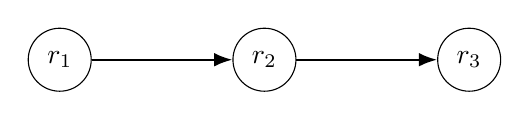
\begin{tikzpicture}[
  >=Latex,
  v/.style={
    circle,
    draw,
    minimum size=8mm,
    inner sep=0pt
  },
  ar/.style={->,thick}
]

\node[v] (a) at (-2.6,0) {$r_1$};
\node[v] (b) at (0,0) {$r_2$};
\node[v] (c) at (2.6,0) {$r_3$};

\draw[ar] (a)--(b);
\draw[ar] (b)--(c);

\end{tikzpicture}

\caption{
read を頂点、overlap を有向辺として表した OLC グラフの例。
}
\label{fig:olc_simple}
\end{figure}

先ほどの三つの read は、図\ref{fig:olc_simple}のような OLC グラフになる。接続候補が一意であれば、図\ref{fig:olc_simple}のようにグラフはほぼ一本道になる。しかし、実シーケンシングデータでは repeat、sequencing error、曖昧な overlap などによって複数の接続候補が生じ、分岐や合流が現れる。さらに、複数の辺をたどって元の頂点へ戻る場合にはサイクルが形成される \cite{li2016miniasm,kamath2017hinge,kolmogorov2019flye}。図\ref{fig:olc_complex}は、このような構造を模式的に示している。

% ============================================================
% Figure 3
% ============================================================

\begin{figure}[tbp]
\centering
\begin{tikzpicture}[
  >=Latex,
  v/.style={
    circle,
    draw,
    minimum size=7mm,
    inner sep=0pt
  },
  ar/.style={->,thick}
]

\node[v] (a) at (-3.2,0) {};

\node[v] (b1) at (-1.3,0.8) {};
\node[v] (b2) at (-1.3,-0.8) {};

\node[v] (c1) at (0.8,0.8) {};
\node[v] (c2) at (0.8,-0.8) {};

\node[v] (d) at (3.0,0) {};

\draw[ar] (a)--(b1);
\draw[ar] (a)--(b2);

\draw[ar] (b1)--(c1);
\draw[ar] (b2)--(c2);

\draw[ar] (c1)--(d);
\draw[ar] (c2)--(d);

\draw[ar] (c1)
to[bend left=35] (b1);

\node[
  font=\scriptsize,
  anchor=west
] at (3.55,0.35)
{分岐 / 合流 / サイクル};

\end{tikzpicture}

\caption{
実データの OLC グラフで現れる複雑な構造の模式図。候補 overlap が複数存在すると、一本道ではなく分岐、合流、サイクルが生じる。
}
\label{fig:olc_complex}
\end{figure}

したがって、実際の assembly で問題になるのは read 数だけではない。複数の候補接続を含むグラフから、同じ read を不適切に繰り返し使用せず、全体として整合的な経路を選ぶ必要がある。特に重要なのは、サイクルを含むかどうかによって経路探索の計算量が大きく変わることである。


% ============================================================
\subsection{DAG とサイクルを含むグラフの計算量}
% ============================================================

グラフの頂点数が多いこと自体は、必ずしも計算上の難しさを意味しない。サイクルを含まない有向非巡回グラフ（DAG）では、頂点をトポロジカル順序に並べることで \cite{kahn1962topological}、前の頂点で求めた最適値を次の頂点へ順に伝えられる。そのため、最大重み経路は動的計画法によって厳密に求めることができ、計算量は
\[
T_{\mathrm{DAG}}=O(|V|+|E|)
\]
である。したがって、頂点数が大きくても、その部分が DAG であれば古典計算で効率よく処理できる。

一方、サイクルを含む一般の有向グラフでは、同じ頂点を二度使用しないという条件を保ちながら最適な経路を選ぶ必要がある。DAG のように一つの順序に沿って各頂点を一度ずつ処理することはできず、問題は組合せ最適化になる。サイクル部分に含まれる頂点数を $k$ とすると、例えばハミルトニアン経路やハミルトニアンサイクルに対する代表的な部分集合動的計画法では、計算量は
\[
T_{\mathrm{cycle}}=O(k^2 2^k)
\]
程度、必要なメモリは概ね $O(k2^k)$ となる。したがって、サイクル部分が十分小さければ古典的な厳密解法でも処理できるが、$k$ が増えると必要な計算資源は急速に増大する。



\begin{table}[tbp]
\centering
\begin{tabular}{|c|c|c|}
\hline
\textbf{グラフ構造}
& \textbf{古典解法}
& \textbf{計算量}
\\ \hline

DAG
& 動的計画法
& $O(|V|+|E|)$
\\ \hline

小規模なサイクル部分
& 部分集合動的計画法 / 厳密解法
& $O(k^2 2^k)$ 程度
\\ \hline

大規模なサイクルを含むグラフ
& 組合せ最適化
& 指数関数的に増大
\\ \hline

\end{tabular}

\caption{
DAG とサイクルを含むグラフに対する古典計算の違い。$k$ はサイクル部分に含まれる頂点数を表す。
}
\label{tab:dag_cycle_complexity}
\end{table}

この違いを表\ref{tab:dag_cycle_complexity}にまとめる。表\ref{tab:dag_cycle_complexity}が示すように、本研究で計算上のボトルネックとなるのはグラフ全体ではなく、DAG として切り離せずに残るサイクル部分である。この違いから、大規模な OLC グラフを一つの方法で処理するのではなく、構造に応じて解法を分ける方針が自然に導かれる。


% ============================================================
\subsection{古典計算と量子最適化の役割分担}
% ============================================================

DAG 部分を古典計算で厳密に解けるなら、量子アニーリングをグラフ全体へ適用する必要はない。本研究では、まず DAG 部分をできるだけ分離して動的計画法で処理し、そこから切り離せないサイクル部分だけを局所的な最適化問題として残す。小さなサイクル部分は古典的な厳密解法でも扱えるが、組合せが大きくなる部分については QUBO、SQA、QA の対象とする。したがって、グラフ圧縮の目的は単に頂点数を減らすことではなく、組合せ最適化が必要な部分をできるだけ小さく局所化することにある。

次章では、まず既存のグラフアルゴリズムと QUBO 定式化を用いて DNA assembly をどこまで処理できるかを復現実験によって確認する。その結果から明らかになる限界を踏まえ、第4章では小さなサイクル問題を量子アニーリングで扱うためのハミルトニアンを構成し、第5章では大規模な実データのグラフをその規模まで縮約するグラフ圧縮法を説明する。

% ============================================================
\section{量子アニーリングによる DNA assembly の先行研究と再現結果}
% ============================================================

既存研究では、DNA assembly を QUBO に写像し、量子アニーリングによって
read の並びを探索する方法が提案されている。ここで重要なのは、小規模な例で
正しい配列を得られるかだけではない。どの制約が正しい read layout の選択に
寄与しているのか、また、その情報を実シーケンシングデータへ拡張したときに
何が計算上のボトルネックとなるのかを区別する必要がある。

そこで本章では、まず Boev \textit{et al.} の定式化を基準として既存研究を
整理する。続いて、その DAG 型定式化を出発点とした制御実験を行い、
経路構造、再構成長、GC 組成、overlap の情報量という異なる情報が
read layout の選択にどのように作用するかを比較する。


% ============================================================
\subsection{既存の QUBO 定式化とその限界}
% ============================================================

Boev \textit{et al.} は、OLC グラフ上で read の順序を求める問題を
ハミルトン経路問題として表し、QUBO に変換して D-Wave および
量子インスパイアード・アニーリングで解いた \cite{boev2021genome}。
$N$ 個の read からなる OLC グラフを $G=(V,E)$ とし、
read $v$ が経路上の $i$ 番目に置かれるとき $x_{v,i}=1$ とする。
このとき、各 read を一度だけ使うこと、各位置に一つの read だけを置くこと、
OLC グラフに存在しない接続を選ばないことを、

\begin{equation}
\begin{aligned}
H_{\mathrm{Boev}}
={}&
A\sum_{v=1}^{N}
\left(
1-\sum_{i=1}^{N}x_{v,i}
\right)^2
+
A\sum_{i=1}^{N}
\left(
1-\sum_{v=1}^{N}x_{v,i}
\right)^2
\\
&+
A\sum_{(u,v)\notin E}
\sum_{i=1}^{N-1}
x_{u,i}x_{v,i+1}
\end{aligned}
\label{eq:boev_hamiltonian}
\end{equation}

によって表す。最初の二項は read と位置の一対一対応を課し、
最後の項は OLC グラフに存在しない read 対が経路上で隣接することを抑える。
したがって、これらの制約を満たす低エネルギー状態から
OLC グラフ上のハミルトン経路を読み出すことができる。

この位置変数型の定式化では、read と位置の組ごとに二値変数が必要となるため、
$N$ reads に対して $N^2$ 個の論理変数を用いる。
Boev \textit{et al.} は、候補グラフが DAG の場合には候補辺そのものを
二値変数として扱うことで、変数数を $|E|$ まで減らせることも示している。
一方、第2章で述べたように、DAG 上の最長経路は動的計画法によって
厳密に求めることができる。したがって、DAG 化によって QUBO が小さくなることと、
量子アニーリングで処理すべき組合せ最適化が残ることは分けて考える必要がある。

実データへ進むと、グラフの規模だけでなく、repeat や orientation の曖昧さに由来する
branch、merge、サイクルも現れる。Boev \textit{et al.} の
$\phi$X174 を用いた計算では、既知の reference genome から人工的に生成した
50 本の read を用い、read 長 600 bp、sequencing error を含まない条件で
検証している \cite{boev2021genome}。
QuASeR でも de novo assembly の QUBO 化と D-Wave による配列再構成が検討され
\cite{sarkar2021quaser}、Nalecz-Charkiewicz and Nowak は sequencing error を
考慮するため、DNA 配列を信号として扱い、read 間のピアソン相関を利用した
定式化を提案している \cite{nalecz2022assembly}。

これらの研究によって、DNA assembly を量子最適化問題として記述できることは
示されている。一方、実シーケンシングデータから生じる大規模な cyclic OLC グラフを
どのように縮約し、どの部分を量子最適化へ渡すべきかという問題は残る。
その前に、経路構造だけを QUBO に与えた場合に何の情報が不足するのかを
明確にしておく必要がある。そこで次に、各情報を一つずつ加えた制御実験を行う。


% ============================================================
\subsection{制御実験で用いたハミルトニアン}
% ============================================================

本節の数値実験では、先行研究で用いられている DAG 上の edge-variable 表現を
出発点とし、候補 overlap 辺そのものを二値変数として扱った。
候補辺 $(i,j)\in E$ について、

\[
x_{ij}
=
\begin{cases}
1, & r_i\text{ の後に }r_j\text{ を接続する場合},\\
0, & \text{それ以外}
\end{cases}
\]

とする。

まず、選択された辺が一本の経路を構成するための基本条件を $H_A$ にまとめる。
$N$ 個の read をすべて通る経路には $N-1$ 本の辺が必要である。
また、一つの read に複数の predecessor や successor が接続すると
一本の read layout にはならない。頂点 $v$ への候補入辺を $\delta^-(v)$、
候補出辺を $\delta^+(v)$ とすると、実装で用いた構造項は

\begin{equation}
\begin{aligned}
H_A
={}&
A
\left(
\sum_{e\in E}x_e-(N-1)
\right)^2
\\
&+
A\sum_{v\in V}
\sum_{\substack{e,f\in\delta^-(v)\\e<f}}
x_e x_f
+
A\sum_{v\in V}
\sum_{\substack{e,f\in\delta^+(v)\\e<f}}
x_e x_f .
\end{aligned}
\label{eq:H_A_path}
\end{equation}

第一項は選択辺数を $N-1$ にそろえ、後二項は各頂点の入次数と出次数が
1 を超える状態にペナルティを与える。本実験で用いる候補グラフは DAG であるため、
これらの条件を同時に満たす状態は、全 read を結ぶ一本のハミルトン経路となる。

しかし、$H_A$ が指定するのは主として経路の構造であり、
複数のハミルトン経路が存在するときに、どの経路が元の DNA に対応するかを
十分に区別できるとは限らない。そこで、assembly 全体に関する情報を
追加したときに選択がどのように変わるかを調べた。

read $r_i$ の長さを $\ell_i=|r_i|$、$r_i$ の末尾と $r_j$ の先頭との
overlap 長を $O_{ij}$ とする。選択した辺から得られる assembly length は

\[
L_{\mathrm{asm}}(\boldsymbol{x})
=
\sum_{i=1}^{N}\ell_i
-
\sum_{(i,j)\in E}O_{ij}x_{ij}
\]

である。目標とする DNA 長を $L_{\mathrm{target}}$ とし、

\begin{equation}
H_B
=
B
\left[
L_{\mathrm{asm}}(\boldsymbol{x})
-
L_{\mathrm{target}}
\right]^2
\label{eq:H_length_abcd}
\end{equation}

とした。この項は、個々の overlap を独立に評価するのではなく、
選択された overlap 全体が一つの assembly として整合する長さを与えるかを評価する。

次に、assembly の塩基組成を用いる。read $r_i$ に含まれる G と C の総数を
$g_i$、辺 $(i,j)$ が表す overlap 部分の GC 数を
$g_{ij}^{\mathrm{ov}}$ とすると、

\[
G_{\mathrm{asm}}(\boldsymbol{x})
=
\sum_{i=1}^{N}g_i
-
\sum_{(i,j)\in E}g_{ij}^{\mathrm{ov}}x_{ij}
\]

である。目標 GC 比率を $p_{\mathrm{GC}}$ として、

\begin{equation}
H_C
=
C
\left[
G_{\mathrm{asm}}(\boldsymbol{x})
-
p_{\mathrm{GC}}
L_{\mathrm{asm}}(\boldsymbol{x})
\right]^2
\label{eq:H_gc_abcd}
\end{equation}

を用いた。これにより、同程度の assembly length を持つ候補の間で、
配列全体の GC 組成との整合性を比較できる。

最後に、overlap alignment そのものが持つ情報を局所的な辺の評価として加えた。
本実装では、辺 $(i,j)$ の normalized mutual information を
$\mathrm{NMI}_{ij}$ とし、overlap 長を掛けた

\[
w_{ij}^{\mathrm{MI}}
=
O_{ij}\mathrm{NMI}_{ij}
\]

を辺 score とした。情報量の高い overlap を選ぶほどエネルギーが下がるよう、

\begin{equation}
H_D
=
-D
\sum_{(i,j)\in E}
w_{ij}^{\mathrm{MI}}x_{ij}
\label{eq:H_mi_abcd}
\end{equation}

とする。

したがって、比較するハミルトニアンは

\begin{equation}
H
=
H_A+H_B+H_C+H_D
\label{eq:abcd_total}
\end{equation}

を基本形とし、$B,C,D$ を個別に 0 とすることで
$A$、$A+B$、$A+C$、$A+D$、$A+B+C$、$A+B+D$、
$A+B+C+D$ を同じデータ上で比較した。


% ============================================================
\subsection{人工データと数値計算の設定}
% ============================================================

各項の効果を分離して調べるため、最初の ablation では
ground truth が既知の人工 DNA を用いた。
長さ $20\,000$、$22\,500$、$25\,000$ bp の線形 DNA を独立に生成し、
各配列から長さ $3\,000$ bp の read を 500 bp 間隔で切り出した。
したがって隣接 read の真の overlap 長は $2\,500$ bp であり、
三つのデータセットにはそれぞれ 35、40、45 本の read が含まれる。
この段階では mismatch、insertion、deletion は加えず、
入力 read の順序のみをシャッフルした。

read から直接正解辺を作るのではなく、実際の OLC pipeline と同様に
minimap2 によって overlap candidate を探索し、その候補を Parasail による
semi-global alignment で再評価した。これにより得られた候補辺数は、
35、40、45 reads に対してそれぞれ 131、151、172 本であった。
一つの候補辺に一つの QUBO 変数を割り当てるため、論理変数数も同じである。

主要な実験条件を表~\ref{tab:abcd_setup} にまとめる。

\begin{table}[t]
\centering
\caption{A/B/C/D ablation に用いた人工データと SQA の主要条件。}
\label{tab:abcd_setup}
\begin{tabular}{ll}
\hline
項目 & 設定 \\
\hline
人工 genome length & $20\,000,\ 22\,500,\ 25\,000$ bp \\
DNA 生成時 GC parameter & $0.5$ \\
simulation seed & $42$ \\
read length & $3\,000$ bp \\
read step & $500$ bp \\
read 数 & $35,\ 40,\ 45$ \\
mismatch / insertion / deletion & $0/0/0$ \\
candidate search & minimap2 \texttt{ava-ont} \\
minimum overlap & $500$ bp \\
overhang tolerance & $80$ bp \\
refinement & Parasail semi-global alignment \\
refinement max error rate & $0.20$ \\
candidate edges & $131,\ 151,\ 172$ \\
solver & OpenJij SQA \\
SQA samples per run & $100$ \\
Monte Carlo sweeps & $1000$ \\
Trotter slices & $32$ \\
annealer seeds & $40,\ 41$ \\
$A$ & $100$ \\
$B$ & $10^{-6}$ \\
$C$ & $10^{-4}$ \\
$D$ & $0.01$ \\
\hline
\end{tabular}
\end{table}

$H_B$ の $L_{\mathrm{target}}$ には生成した人工 genome の真の長さを用いた。
同様に、$H_C$ の $p_{\mathrm{GC}}$ には生成後の genome から直接計算した
GC 比率を用いた。したがって、この実験は未知 DNA の de novo assembly を
そのまま模擬するものではなく、各ハミルトニアン項が探索に与える効果を
分離するための controlled benchmark として位置づけられる。

SQA の結果は、人工データが持つ true genome coordinate から既知の
reference read order を作り、その経路を QUBO に代入した energy と比較した。
SQA sample の energy が reference path の energy と $10^{-6}$ 未満で一致した場合を、
以下では reference-energy hit とする。さらに、選択辺数、入次数・出次数制約、
および真の隣接 read edge が回収されているかも同時に確認した。


% ============================================================
\subsection{再現実験から分かったこと}
% ============================================================

まず、どの情報が正しい read layout の選択に寄与したかを比較する。
35、40、45 reads の各データセットについて二つの annealer seed を用いたため、
各ハミルトニアンにつき計 6 runs を評価した。結果を
表~\ref{tab:abcd_ablation} に示す。

\begin{table}[t]
\centering
\caption{35、40、45 reads の人工データに対する A/B/C/D ablation。
各条件は 3 データサイズ $\times$ 2 annealer seeds の計 6 runs である。}
\label{tab:abcd_ablation}
\begin{tabular}{lc}
\hline
Hamiltonian & reference-energy hits \\
\hline
旧 edge-path DAG & $1/6$ \\
$A$ & $0/6$ \\
$A+B$ & $\mathbf{6/6}$ \\
$A+C$ & $0/6$ \\
$A+D$ & $0/6$ \\
$A+B+C$ & $4/6$ \\
$A+B+D$ & $5/6$ \\
$A+B+C+D$ & $\mathbf{6/6}$ \\
\hline
\end{tabular}
\end{table}

最も明確な変化は、$A$ に assembly length の情報 $B$ を加えたときに現れた。
$A$ のみでは $0/6$ であったのに対し、$A+B$ では 6 runs すべてで
reference energy に到達した。さらに、この 6 runs では選択辺数が
すべて $N-1$ となり、入次数・出次数の violation は 0、
真の隣接 read edge もすべて回収された。したがって、本実験の範囲では
$A+B$ が正しい read layout を一貫して再現した最小の構成である。

この違いは、$B$ 項がこの人工データに対して持つ役割を見ると理解しやすい。
例えば 35 reads の場合、各 read は $3\,000$ bp であるため、

\[
\sum_{i=1}^{35}\ell_i
=
105\,000\ {\rm bp}
\]

である。一方、target genome length は $20\,000$ bp である。
したがって $H_B=0$ となるためには、

\[
\sum_e O_e x_e
=
105\,000-20\,000
=
85\,000\ {\rm bp}
\]

が必要となる。さらに $H_A$ は 34 本の辺を選択するため、
選択辺あたりの平均 overlap は

\[
\frac{85\,000}{34}
=
2\,500\ {\rm bp}
\]

となる。これは、この人工データにおける真の隣接 read の overlap 長
$3\,000-500=2\,500$ bp と一致する。

したがって、この controlled benchmark では $B$ 項は単に
``assembly length を合わせる'' だけでなく、選択された overlap 全体の総量を
一つの大域的条件で拘束している。$A$ が経路の形を定め、$B$ がその経路全体の
overlap 総量を制約することで、多数の構造的に可能な経路の中から
真の read order に整合する候補が強く選択されたと解釈できる。
$A+B$ の成功率が $A$ のみの場合から大きく改善したという観測は、
この機構と整合している。

一方、$A+C$ と $A+D$ はいずれも $0/6$ であり、
$A+B+C$ と $A+B+D$ も $A+B$ を一貫して上回らなかった。
したがって、利用可能な情報を追加するだけで SQA の結果が単調に改善するわけではない。
今回の人工 DNA はほぼ一様なランダム配列として生成されているため、
GC composition は異なる経路を区別する情報として弱かった可能性がある。
また、$D$ は各 overlap を局所的に評価するため、一本の assembly 全体の整合性を
直接指定する $B$ とは役割が異なる。これらは数値結果から考えられる解釈であり、
各項が energy landscape や SQA の遷移に与える影響を分離するには
さらに詳細な解析が必要である。

$B$ の効果は 35--45 reads のみに限った観測ではなかった。
別の人工データ系列では、GC parameter を $0.65$ として read 数を増やした場合にも
$A+B$ は高い再現率を維持し、80、90、100 reads の比較では計 6 runs すべてで
reference energy に到達したのに対し、従来の edge-path DAG Hamiltonian は
同じ 6 runs で reference energy に到達しなかった。
さらに 200 reads、798 edge variables の多 seed 計算では、
10 runs すべてで reference-energy hit、valid path、DNA recoverability が確認された。
70 reads に mismatch、insertion、deletion を含む人工誤差を加えた追加実験でも、
$A+B$ は 2--5\% の tested error regime で reference-energy hit を維持した。
一方、$D$ の追加による一貫した改善は、この範囲では確認されていない。
これらの追加計算は、初期 ablation で観測された $B$ の効果が
一つの 35-read instance に限られたものではないことを支持している。

ただし、この結果を実シーケンシングデータへ移す際には、
controlled benchmark で用いた条件を明確に分ける必要がある。
第一に、$H_B$ は $L_{\mathrm{target}}$ を必要とする。
今回の計算では simulator が生成した genome の真の長さを利用したが、
未知 genome の de novo assembly では同じ精度の事前情報を常に利用できるとは限らない。
$H_C$ に用いた GC 比率についても同様である。

第二に、本実験の候補グラフは DAG として処理できる構造である。
DAG 上の最長経路は古典的な動的計画法によって厳密に求められるため、
この結果自体は量子最適化が必要なサイクル問題を解いたことを意味しない。
本実験の役割は、量子優位性を示すことではなく、
どの情報が QUBO 上で正しい read layout を選ぶために有効かを切り分ける点にある。

第三に、今回の $A$ 項には

\[
\left(
\sum_e x_e-(N-1)
\right)^2
\]

という大域的な edge-count constraint が含まれており、この項を展開するだけでも
異なる edge variables の間に二次結合が生じる。
$B$ や $C$ も同様に assembly 全体を参照する二次形式であるため、
候補辺数が大きくなると多数の変数が相互作用する。
したがって、小規模な人工 DAG で有効なハミルトニアンを
大規模な実 OLC グラフへそのまま拡張するよりも、
まずグラフの構造を利用して本当に組合せ最適化が必要な領域を限定することが重要となる。

以上の再現実験から、実データへ進むための二つの課題が見えてくる。
一つは、大規模な OLC グラフから古典計算で処理できる DAG 部分を分離し、
サイクルを含む曖昧な領域だけを小さな最適化問題として残すことである。
もう一つは、その局所問題に対して genome 全体の真の長さのような
強い大域情報に依存せず、サイクル構造そのものを扱えるハミルトニアンを構成することである。

次章では後者の問題から取り組み、小さな cyclic OLC グラフを
量子アニーリングで扱うためのハミルトニアンを構成する。
その後、第5章では、大規模な実シーケンシングデータから
この局所的な cyclic problem を取り出すためのグラフ圧縮法を説明する。






















% ============================================================
% ============================================================
\section{循環 OLC グラフに対する QUBO アルゴリズム}
% ============================================================

第3章では、候補辺を二値変数とする QUBO を用いて read の並びを求めた。
候補グラフが DAG であれば、各頂点の入次数と出次数、および選択する辺の本数を制約することで、
選択された辺は一本の Hamilton path になる。
しかし、実際の OLC グラフには repeat などに由来するサイクルが含まれる。
本章では、第3章の辺変数型 QUBO を循環グラフへ拡張する方法を検討する。

% ============================================================
\subsection{循環グラフで生じる問題と評価データ}
% ============================================================

% TODO: 第3章の weighted edge-variable QUBO を確定した後、その式をここで参照し、
% 本章で用いる基本 Hamiltonian を H_0 と定義する。
候補辺 $e=(u,v)\in E$ を選ぶとき $x_e=1$、選ばないとき $x_e=0$ とする。
第3章の辺変数型 QUBO では、各頂点の入次数と出次数を 1 以下に抑え、
選択辺数を $N-1$ とすることで経路構造を表した。
DAG ではサイクルが存在しないため、これらの条件を満たす選択辺は全頂点を通る一本の経路になる。

循環グラフでは同じ議論は成立しない。
各頂点の入次数と出次数がともに 1 以下であるとき、選択された辺からなるグラフは、
互いに交わらない有向経路と有向サイクルに分解できる。
選択辺数が $N-1$ となるとき、有向経路は一本になるが、これとは別にサイクルが残る場合がある。
したがって、第3章の制約だけではこの状態と Hamilton path を区別できない。

本章の数値評価には、CHM13 v1.1 の HiFi primary-alignment data から抽出した
144 本の read を用いる。
対象は chr2 の約 89.6--91.2 Mb に対応する区間であり、全 read 対の overlap 計算から得られた
グラフのうち、大きな強連結成分を含む区間を選択した。
候補 overlap は一致率 98\% 以上、overlap 長 300 bp 以上の suffix-to-prefix 接続に限定し、
同一 read 対に複数の候補がある場合は後述の重みが最大となるものを残した。
さらに、98\% 以上の一致率で他の read に完全包含される 9 本を除外した。
read の向きは CHM13 参照配列への primary alignment の鎖方向に合わせて統一した。

最終的な OLC グラフは 144 頂点と 261 本の有向辺からなり、
2 頂点以上を含む強連結成分は 112 頂点と 11 頂点の二つである。
全 Hamilton path を厳密に列挙すると 192 通り存在するため、
単一の回り道だけでなく、複数の分岐が組み合わさった評価例になっている。

辺の重みには参照配列上の位置を用いず、read 間のアラインメントだけを用いる。
辺 $e$ の一致塩基数を $M_e$、アラインメントブロック長を $B_e$、
$d_e=B_e-M_e$ とすると、
\begin{equation}
w_e=M_e-49d_e
\label{eq:complex144_weight}
\end{equation}
とする。
これは一致率 98\% を基準とした品質余裕を整数化したものであり、
長い overlap であっても誤りが多い辺の重みが過大にならないようにしている。
この重みに対して 192 通りの Hamilton path を列挙した結果、
最大値は 1,343,093、次点は 1,338,209 であった。

% TODO: complex144 のグラフ図に差し替える。
\begin{figure}[htbp]
\centering
\fbox{\parbox[c][48mm][c]{0.88\linewidth}{\centering
CHM13 complex144 の OLC グラフ\\[2mm]
144 本の read、261 本の候補辺、主要な強連結成分と分岐を表示する。}}
\caption{CHM13 complex144 の OLC グラフ。}
\label{fig:complex144_topology_placeholder}
\end{figure}

% ============================================================
\subsection{順序変数を用いた QUBO}
% ============================================================

サイクルを QUBO の制約として直接排除する方法として、経路上の順序を補助変数で表す方法がある。
N{\"u}{\ss}lein \textit{et al.}\ \cite{nusslein2022qubo} は Hamiltonian cycle に対し、
候補辺 $(a,b)$ に整数 $P_{ab}$ を割り当て、$P_{ab}=0$ を未選択、
$P_{ab}>0$ をサイクル上の位置として表す定式化を示した。
$P_{ab}$ は
\begin{equation}
P_{ab}
=
\sum_{k=0}^{K-1}2^k p_{ab,k},
\qquad
K=\left\lceil\log_2(N+1)\right\rceil
\label{eq:nusslein_binary_order}
\end{equation}
と二進展開される。
例えば、選択された二辺 $(a,b)$ と $(b,c)$ が連続するときには
\begin{equation}
P_{bc}=P_{ab}+1
\label{eq:nusslein_successive_order}
\end{equation}
を要求し、その差は
\begin{equation}
\left(P_{bc}-P_{ab}-1\right)^2
\label{eq:nusslein_successive_square}
\end{equation}
のような二乗項で表せる。
実際の Hamiltonian では未選択辺にこの条件を課さないための条件付けと、
cycle の端点を接続するための境界条件も加わる。
この方法では、選択した辺の順序を QUBO の内部で同時に決めることによって部分サイクルを排除する。

本研究で必要なのは Hamiltonian cycle ではなく、始点と終点を持つ Hamilton path である。
また、サイクルを排除するためには、選択辺の位置が必ず 1 ずつ連続する必要はない。
そこで、各 read $v$ に順位値 $P_v$ を持たせ、選択した辺 $(u,v)$ に対して
\begin{equation}
x_{uv}=1
\quad\Longrightarrow\quad
P_u<P_v
\label{eq:strict_rank_condition}
\end{equation}
のみを要求する。
選択辺の中に
$v_1\rightarrow v_2\rightarrow\cdots\rightarrow v_L\rightarrow v_1$
というサイクルがあれば、
$P_{v_1}<P_{v_2}<\cdots<P_{v_L}<P_{v_1}$ が必要となるため、
式~\eqref{eq:strict_rank_condition} を満たすことはできない。

以下、この条件を二次式だけで表す。
まず、各 read $v$ の順位値を
\begin{equation}
P_v
=
\sum_{k=0}^{K-1}2^k p_{v,k},
\qquad
p_{v,k}\in\{0,1\},
\qquad
K=\left\lceil\log_2N\right\rceil
\label{eq:latent_vertex_rank}
\end{equation}
とする。

候補辺 $e=(u,v)$ ごとに、$P_v-P_u-1$ の二進減算を行うための
桁借り変数 $b_{e,k}$ を導入する。
$b_{e,k}$ は第 $k$ 桁へ入る桁借り、$b_{e,k+1}$ は第 $k$ 桁から出る桁借りを表し、
$-1$ を含めるため最下位桁への入力を
\begin{equation}
b_{e,0}=1
\end{equation}
と固定する。
第 $k$ 桁では $p_{v,k}$ から $p_{u,k}+b_{e,k}$ を引くので、
\begin{equation}
b_{e,k+1}=1
\quad\Longleftrightarrow\quad
p_{u,k}+b_{e,k}>p_{v,k}
\label{eq:borrow_relation}
\end{equation}
である。

二値変数 $a,d,b,c$ に対し、
\begin{equation}
R(a,d,b,c)
=
a+b+c+ab-ad-bd-2ac-2bc+2dc
\label{eq:borrow_quadratic_penalty}
\end{equation}
とおく。
ここで
\[
a=p_{u,k},\qquad
d=p_{v,k},\qquad
b=b_{e,k},\qquad
c=b_{e,k+1}
\]
である。
式~\eqref{eq:borrow_relation} を満たす $c$ を選んだときに限って $R=0$ となるため、
全候補辺の全 bit に対する桁借り制約は
\begin{equation}
H_{\mathrm{cmp}}
=
A_{\mathrm{cmp}}
\sum_{e=(u,v)\in E}
\sum_{k=0}^{K-1}
R\!\left(
p_{u,k},p_{v,k},b_{e,k},b_{e,k+1}
\right)
\label{eq:comparator_hamiltonian}
\end{equation}
と書ける。
$b_{e,0}$ は定数 1 であり、実際に追加する桁借り変数は
$b_{e,1},\ldots,b_{e,K}$ の $K$ 個である。

最上位桁まで減算した後、
\begin{equation}
b_{e,K}=1
\quad\Longleftrightarrow\quad
P_v\leq P_u
\label{eq:final_borrow_order}
\end{equation}
となる。
したがって、選択した辺だけについて最終桁借りを禁止する
\begin{equation}
H_{\mathrm{ord}}
=
A_{\mathrm{ord}}
\sum_{e=(u,v)\in E}
x_e b_{e,K}
\label{eq:strict_rank_gate}
\end{equation}
を加えると、式~\eqref{eq:strict_rank_condition} が得られる。

次に Hamilton path の始点と終点を表す。
頂点 $v$ が始点であるとき $s_v=1$、終点であるとき $t_v=1$ とする。
各頂点について
\begin{equation}
H_{\mathrm{deg}}
=
A_{\mathrm{deg}}
\sum_{v\in V}
\left[
\left(
1-s_v-\sum_{u:(u,v)\in E}x_{uv}
\right)^2
+
\left(
1-t_v-\sum_{w:(v,w)\in E}x_{vw}
\right)^2
\right]
\label{eq:strict_rank_degree_hamiltonian}
\end{equation}
とすれば、始点以外では入辺を一本、終点以外では出辺を一本選ぶことになる。
始点と終点をそれぞれ一つに限定し、同じ頂点を両方に選ぶ状態を除くため、
\begin{equation}
\begin{aligned}
H_{\mathrm{end}}
={}&
A_{\mathrm{end}}
\left[
\left(1-\sum_{v\in V}s_v\right)^2
+
\left(1-\sum_{v\in V}t_v\right)^2
\right]
\\
&+
A_{\mathrm{diff}}
\sum_{v\in V}s_vt_v
\end{aligned}
\label{eq:strict_rank_endpoint_hamiltonian}
\end{equation}
を加える。

最後に overlap の重みを目的関数へ入れる。
式~\eqref{eq:complex144_weight} の $w_e$ を用い、
\begin{equation}
c_e
=
\frac{w_{\max}-w_e}
{\max_{f\in E}(w_{\max}-w_f)}
\label{eq:strict_rank_edge_cost}
\end{equation}
と規格化した非負コストを定義する。
Hamilton path では選択辺数が常に $N-1$ であるため、
$\sum_e c_ex_e$ の最小化は $\sum_e w_ex_e$ の最大化と同じ順位を与える。
よって
\begin{equation}
H_{\mathrm{weight}}
=
A_{\mathrm{weight}}
\sum_{e\in E}c_ex_e
\label{eq:strict_rank_weight_hamiltonian}
\end{equation}
とする。

以上を合わせ、本節で用いる順位比較型 QUBO は
\begin{equation}
H_{\mathrm{rank}}
=
H_{\mathrm{weight}}
+
H_{\mathrm{deg}}
+
H_{\mathrm{end}}
+
H_{\mathrm{cmp}}
+
H_{\mathrm{ord}}
\label{eq:strict_rank_total}
\end{equation}
である。
式~\eqref{eq:strict_rank_degree_hamiltonian} と
式~\eqref{eq:strict_rank_endpoint_hamiltonian} が一本の開いた経路の次数条件を与え、
式~\eqref{eq:comparator_hamiltonian} と式~\eqref{eq:strict_rank_gate} が
その経路にサイクルが含まれないことを保証する。

% ============================================================
\subsection{順序変数 QUBO の規模と予備検証}
% ============================================================

complex144 では $N=144$、$M=261$ であり、一頂点あたりの順位ビット数は $K=8$ となる。
式~\eqref{eq:strict_rank_total} では、261 個の辺変数、288 個の始点・終点変数、
1152 個の順位ビット、2088 個の桁借り変数を用いる。したがって論理変数数は
\begin{equation}
Q=M+2N+NK+MK=3789
\label{eq:strict_rank_variable_count}
\end{equation}
となる。

N{\"u}{\ss}lein \textit{et al.} の構成に基づく辺位置型 QUBO では、
二進展開した位置値を二乗制約に含めるため、上位 bit の係数が二次項で大きくなる。
complex144 に対して実装した場合、最大二次係数は約 $9.44\times10^6$ であった。
これに対し、式~\eqref{eq:borrow_quadratic_penalty} の桁借りを用いた順位比較では、
各 bit の関係を小さい整数係数で表せる。
表~\ref{tab:order_qubo_comparison} に両者の QUBO 規模を示す。

\begin{table}[htbp]
\centering
\caption{complex144 に対する順序変数 QUBO の規模。}
\label{tab:order_qubo_comparison}
\begin{tabular}{lrrr}
\hline
定式化 & 論理変数数 & 二次結合数 & 最大二次係数 \\
\hline
辺位置型 & 2637 & 77843 & 9437184 \\
順位比較型 & 3789 & 33376 & 576 \\
\hline
\end{tabular}
\end{table}

まず、既知の Hamilton path を二値変数へ符号化し、各制約を個別に確認した。
次数、始点・終点、各桁の桁借り、選択辺の順位関係はいずれも違反数 0 となった。
また、同じ頂点順序に対して順位値を連続に与えた場合、全順位を一定値だけずらした場合、
順位間隔を不均一にした場合で目的関数値は変化しなかった。
この結果から、順位比較型 QUBO が順位の絶対値ではなく前後関係だけを用いて
Hamilton path を表していることを確認した。

定式化の基本的な挙動を確認するため、QBSolv による予備計算も行った。
基準のペナルティ設定では 135--138 本の辺が選択され、桁借り制約の違反は 0 であったが、
次数制約と選択辺の順位関係には違反が残った。
順位違反のペナルティを強くすると順位関係は満たされる一方、
選択辺数は約 80--83 本まで減少し、全頂点を結ぶ経路にはならなかった。

順位比較型では大きな二次係数を避けられるが、
261 本の候補辺を扱うために 3789 個の論理変数を探索する必要がある。
また、経路の一部をつなぎ替えると、対応する辺変数だけでなく、
順位 bit と各候補辺の桁借り変数も整合する値へ変化しなければならない。
この補助変数の更新を QUBO 探索に含めることが、次に小規模化すべき部分である。
正式な solver 比較は第4.5節の条件で行う。

% ============================================================
\subsection{辺変数 QUBO とサイクル情報による反復更新}
% ============================================================

順位変数と桁借り変数を QUBO から除き、候補辺 $x_e$ だけを探索変数とする。
本節では、第3章で用いた辺変数型の構造項に
式~\eqref{eq:complex144_weight} の overlap 重みを加えたものを
基本 Hamiltonian $H_0$ とする。
% TODO: 第3章改稿後、H_0 は第3章の該当式を直接参照する。
概念的には
\begin{equation}
H_0
=
H_{\mathrm{weight}}
+
H_{\mathrm{degree}}
+
H_{\mathrm{count}}
\label{eq:edge_only_base_hamiltonian}
\end{equation}
であり、complex144 では 261 個の辺変数だけを用いる。

$H_0$ だけでは、第4.1節で述べた経路とサイクルの共存を排除できない。
一方、ある $x_e$ が与えられた後に、その選択辺からなるグラフがサイクルを含むかどうかを調べることは容易である。
強連結成分の分解や有向サイクルの検出は $O(|V|+|E|)$ のグラフ探索で実行できる。
そこで、QUBO の中に全頂点の順位を保持する代わりに、QUBO を一度解いた後で
サイクルを古典計算によって検出し、その情報を次の QUBO に反映する。

第 $t$ 回の求解で得られた選択辺を $x^{(t)}$ とする。
選択辺からなるグラフを強連結成分に分解し、2 頂点以上を含む各強連結成分から
一つの有向サイクルを検出する。
得られたサイクルの集合を $\mathcal{C}^{(t)}$ とする。
サイクル $C$ に含まれるどの辺を外すかはあらかじめ指定せず、
すべての辺に同じ線形ペナルティを与える。
\begin{equation}
H_{\mathrm{cyc}}^{(t)}
=
A_{\mathrm{cyc}}
\sum_{C\in\mathcal{C}^{(t)}}
\sum_{e\in C}x_e
\label{eq:uniform_cycle_penalty}
\end{equation}
この定義では、サイクルの長さによらず各辺を選択することによる追加コストは
$A_{\mathrm{cyc}}$ である。
長いサイクルだけ一辺当たりのペナルティが小さくなることはない。

次回に解く QUBO は
\begin{equation}
H^{(t+1)}
=
H_0+H_{\mathrm{cyc}}^{(t)}
\label{eq:iterative_cycle_hamiltonian}
\end{equation}
とする。
過去に検出したサイクルのペナルティは蓄積せず、
各回の解からサイクルを検出し直して式~\eqref{eq:uniform_cycle_penalty} を作り直す。
したがって論理変数数は 261 のままであり、
順位比較型で用いた順位 bit、桁借り変数、始点・終点変数を探索変数として持たない。

\begin{figure}[htbp]
\centering
\begin{tikzpicture}[
  >=Latex,
  box/.style={draw,rounded corners=1.5mm,minimum width=31mm,minimum height=10mm,align=center,font=\small},
  node distance=12mm and 14mm
]
\node[box] (qubo) {QUBO 求解\\$H^{(t)}$};
\node[box,right=of qubo] (state) {選択された辺\\$x^{(t)}$};
\node[box,right=of state] (check) {古典計算による\\サイクル検出};
\node[box,below=of state] (update) {ペナルティ更新\\$H^{(t+1)}$};
\draw[->,thick] (qubo) -- (state);
\draw[->,thick] (state) -- (check);
\draw[->,thick] (check) |- (update);
\draw[->,thick] (update) -| (qubo);
\end{tikzpicture}
\caption{QUBO 求解と古典的なサイクル検出を交互に行う反復計算。}
\label{fig:iterative_cycle_feedback}
\end{figure}

この方法で反復ごとに変更するのは QUBO の線形係数である。
そのため、各回の QUBO を解く部分は特定の solver に依存せず、
本報告では数値評価のために SQA を用いる。

% ============================================================
\subsection{数値評価の方法}
% ============================================================

順位比較型 QUBO と、サイクル情報を用いて反復更新する辺変数型 QUBO を
complex144 上で比較する。
前者は 3789 論理変数を用い、計算中に Hamiltonian を変更しない。
後者は 261 論理変数を用い、各反復の間に
式~\eqref{eq:iterative_cycle_hamiltonian} に従って線形項を更新する。

計算量をそろえるため、一つの独立試行を両定式化とも 16 回の SQA 呼び出しで構成する。
各呼び出しには OpenJij の SQASampler を用い、
$\beta=5$、$\Gamma=1$、Trotter 数 $P=8$、1400 sweeps、
\texttt{num\_reads}=8 とする。
したがって、一つの独立試行で生成するサンプル数と sweep 数は両定式化で同じである。
各呼び出しで得られた 8 サンプルのうち QUBO エネルギーが最も低い状態を
次回の初期状態とする。

順位比較型では 16 回を通して同一の Hamiltonian を用いる。
反復更新型では各 SQA 呼び出しの後にサイクルを検出し、
式~\eqref{eq:uniform_cycle_penalty} を用いて次回の Hamiltonian を作る。
$A_{\mathrm{cyc}}$ は規格化後の辺コストに対する一定値として正式計算前に固定し、
全試行で同じ値を用いる。
% TODO: 正式計算に用いた A_cyc の値を結果表と同時に記入する。

各定式化について 24 回の独立試行を行う。
SQA が返した全サンプルについて、選択辺が Hamilton path を構成するかを
補助変数とは独立に検査する。
各試行では、得られた Hamilton path の中で最大の重みを記録する。
集計には Hamilton path を一度以上得た試行数、最大重みの中央値と四分位範囲、
全試行中の最大値、既知最適値への到達回数を用いる。
また、順位比較型では制約違反数、反復更新型では各反復で検出されたサイクル数を保存する。
実行時間も記録し、論理変数数の違いが実際の計算時間に与える影響を確認する。

% TODO: 正式計算後に結果表と score 分布を追加する。
% 候補: 論理変数数 / HP取得試行数 / 最大重みの中央値 / IQR /
% 全体最大値 / 最適値到達回数 / 実行時間。


\section{グラフ圧縮法}
% ============================================================

前章では、固定した始点--終点を持つ小さなサイクル問題を QUBO に変換し、
量子アニーリングで扱うためのハミルトニアンを構成した。
次に必要なのは、大規模な実シーケンシングデータの OLC グラフから、
その局所問題をどのように取り出すかである。
DAG 部分は動的計画法で厳密に処理し、
組合せ最適化は循環部分へ集中させる。
本章では、古典計算で確定した局所構造を後から復元できる形でまとめ、
上位グラフから見える自由度を段階的に減らすグラフ圧縮法を説明する。

% ============================================================
\subsection{局所ブロックの圧縮と階層化}
\label{subsec:local_compression}
% ============================================================

大規模な OLC グラフの一部を局所ブロック $B$ とする。
外側のグラフから $B$ を見ると、まず必要になるのは、
どこからブロックへ入り、どこから外へ出るかという境界情報である。
そこで、外部から $B$ へ入る境界頂点集合を
$P_B=\{p_1,p_2,\ldots\}$、
外部へ出る境界頂点集合を
$Q_B=\{q_1,q_2,\ldots\}$ とする。

各入口--出口対 $(p_\alpha,q_\beta)$ について、
ブロック内部だけを通る経路のうち、
その局所問題で用いる経路 score を最大にする経路を求める。
その最適 score を $W_{\alpha\beta}^{B}$、
実際の内部経路を $\Pi_{\alpha\beta}^{B}$ とする。
さらに、$\Pi_{\alpha\beta}^{B}$ が使用する元の physical read の集合を
$R_{\alpha\beta}^{B}$ として保存する。
つまり、$W_{\alpha\beta}^{B}$ は「その局所経路がどれだけ良いか」、
$\Pi_{\alpha\beta}^{B}$ は「内部でどの順に進むか」、
$R_{\alpha\beta}^{B}$ は「どの read を消費するか」を表す。

上位のグラフでは、ブロック内部の多数の頂点を直接扱う代わりに、
これらの情報を持つマクロ状態を入口と出口の間に置く。
同じ入口--出口対を結ぶ候補でも、使用する physical read が異なれば、
上位層で他の経路と競合する条件も変わる。
そのため、使用 read の組が異なる内部解は別のマクロ状態として保持する。
この区別によって、局所的に解いた情報を上位層へ渡した後も、
read を一度だけ使うという全体の制約を追跡できる。

図\ref{fig:graph_compression_overview}(a) は、
一つの局所ブロックをマクロ状態へ置き換える操作を示している。
左側の複雑な内部構造は、各入口--出口対に対応するマクロ状態へまとめられる。
図中の橙色の辺には、$W_{\alpha\beta}^{B}$、
$\Pi_{\alpha\beta}^{B}$、$R_{\alpha\beta}^{B}$ が対応しており、
上位グラフからは一つの「内部解の代理」として扱われる。

\begin{figure}[tbp]
\centering

{\small\bfseries
(a) 一つの局所ブロックをマクロ状態へ置き換える}

\vspace{3mm}

\begin{tikzpicture}[
  >=Latex,
  v/.style={circle,draw,minimum size=4.8mm,inner sep=0pt,fill=white},
  ext/.style={circle,draw=gray!65,minimum size=4.6mm,inner sep=0pt,fill=gray!4},
  bd/.style={circle,draw=orange!85!black,very thick,
             minimum size=5.3mm,inner sep=0pt,fill=orange!7,font=\scriptsize},
  ar/.style={->,thick},
  macro/.style={->,very thick,draw=orange!85!black},
  box/.style={draw=orange!85!black,very thick,rounded corners=2mm},
  infobox/.style={draw=gray!65,rounded corners=1.5mm,fill=gray!3,
                  inner xsep=2.2mm,inner ysep=1.5mm},
  txt/.style={font=\scriptsize}
]

% ----- original block -----
\node[ext] (u1) at (-5.2,1.15) {};
\node[ext] (u2) at (-5.2,-1.15) {};
\node[bd] (p1) at (-4.2,1.15) {$p_1$};
\node[bd] (p2) at (-4.2,-1.15) {$p_2$};

\node[v] (a1) at (-2.9,1.15) {};
\node[v] (a2) at (-2.9,0.00) {};
\node[v] (a3) at (-2.9,-1.15) {};

\node[v] (b1) at (-1.6,1.15) {};
\node[v] (b2) at (-1.6,0.00) {};
\node[v] (b3) at (-1.6,-1.15) {};

\node[bd] (q1) at (-0.2,1.15) {$q_1$};
\node[bd] (q2) at (-0.2,-1.15) {$q_2$};
\node[ext] (v1) at (0.8,1.15) {};
\node[ext] (v2) at (0.8,-1.15) {};

\draw[ar] (u1)--(p1);
\draw[ar] (u2)--(p2);
\draw[ar] (p1)--(a1);
\draw[ar] (p1)--(a2);
\draw[ar] (p2)--(a2);
\draw[ar] (p2)--(a3);
\draw[ar] (a1)--(b1);
\draw[ar] (a2)--(b1);
\draw[ar] (a2)--(b2);
\draw[ar] (a3)--(b2);
\draw[ar] (a3)--(b3);
\draw[ar] (b1)--(q1);
\draw[ar] (b2)--(q1);
\draw[ar] (b2)--(q2);
\draw[ar] (b3)--(q2);
\draw[ar] (q1)--(v1);
\draw[ar] (q2)--(v2);

\node[
  box,
  fit=(p1)(p2)(a1)(a2)(a3)(b1)(b2)(b3)(q1)(q2),
  inner sep=3mm,
  label={[txt,text=orange!85!black]above:局所ブロック $B$}
] {};

% ----- transform arrow -----
\node[font=\Large] at (1.85,0) {$\Longrightarrow$};
\node[txt,align=center] at (1.85,-0.62)
{内部経路を解き\\情報を上位層へ渡す};

% ----- macro representation: preserve all four boundary pairs -----
\node[ext] (lv1) at (2.45,1.25) {};
\node[ext] (lv2) at (2.45,-1.25) {};
\node[bd] (rp1) at (3.15,1.25) {$p_1$};
\node[bd] (rp2) at (3.15,-1.25) {$p_2$};
\node[bd] (rq1) at (6.95,1.25) {$q_1$};
\node[bd] (rq2) at (6.95,-1.25) {$q_2$};
\node[ext] (rv1) at (7.95,1.25) {};
\node[ext] (rv2) at (7.95,-1.25) {};

\draw[ar] (lv1)--(rp1);
\draw[ar] (lv2)--(rp2);

\draw[macro] (rp1)--node[pos=0.50,above=2pt,txt,fill=white,inner sep=0.8pt]
{$M_{11}^{B}$} (rq1);
\draw[macro] (rp2)--node[pos=0.50,below=2pt,txt,fill=white,inner sep=0.8pt]
{$M_{22}^{B}$} (rq2);
\draw[macro] (rp1) to[bend right=24]
node[pos=0.30,above=1pt,txt,fill=white,inner sep=0.8pt]
{$M_{12}^{B}$} (rq2);
\draw[macro] (rp2) to[bend left=24]
node[pos=0.70,below=1pt,txt,fill=white,inner sep=0.8pt]
{$M_{21}^{B}$} (rq1);
\draw[ar] (rq1)--(rv1);
\draw[ar] (rq2)--(rv2);

\node[infobox,txt,align=left,anchor=north west] at (3.25,-2.05)
{各 $M_{\alpha\beta}^{B}$ が保存する情報：\\
評価値 $W_{\alpha\beta}^{B}$，内部経路 $\Pi_{\alpha\beta}^{B}$，使用 read $R_{\alpha\beta}^{B}$};

\end{tikzpicture}

\vspace{11mm}

{\small\bfseries
(b) 解いた局所構造を上位グラフへ渡し、残る循環部分へ同じ操作を適用する}

\vspace{3mm}

\begin{tikzpicture}[
  >=Latex,
  x=1cm,y=1cm,
  v/.style={circle,draw,minimum size=4.4mm,inner sep=0pt,fill=white},
  bd/.style={circle,draw=orange!85!black,very thick,
             minimum size=4.8mm,inner sep=0pt,fill=orange!7,font=\scriptsize},
  ordinary/.style={->,thick},
  macroe/.style={->,very thick,draw=orange!85!black},
  blockbox/.style={draw=orange!85!black,very thick,rounded corners=1.6mm},
  activebox/.style={draw=gray!70,dashed,thick,rounded corners=1.6mm},
  layerbox/.style={draw,rounded corners=2mm,fill=gray!3},
  llab/.style={font=\small\bfseries,anchor=east},
  txt/.style={font=\scriptsize}
]

% ---------- Layer 0 ----------
\draw[layerbox] (-4.75,4.20) rectangle (4.75,5.60);
\node[llab] at (-5.05,4.90) {層 0};

\node[v]  (L0s)  at (-4.05,4.90) {};
\node[bd] (L0p1) at (-3.10,5.23) {$p_1$};
\node[bd] (L0p2) at (-3.10,4.57) {$p_2$};
\node[v]  (L0u1) at (-2.10,5.23) {};
\node[v]  (L0u2) at (-2.10,4.57) {};
\node[bd] (L0q1) at (-1.05,5.23) {$q_1$};
\node[bd] (L0q2) at (-1.05,4.57) {$q_2$};
\node[v]  (L0t)  at (0.05,4.90) {};
\node[v]  (L0c1) at (1.15,5.10) {};
\node[v]  (L0c2) at (2.30,4.42) {};
\node[v]  (L0c3) at (3.45,5.10) {};
\node[v]  (L0y)  at (4.20,4.90) {};

\draw[ordinary] (L0s)--(L0p1);
\draw[ordinary] (L0s)--(L0p2);
\draw[ordinary] (L0p1)--(L0u1);
\draw[ordinary] (L0p1)--(L0u2);
\draw[ordinary] (L0p2)--(L0u1);
\draw[ordinary] (L0p2)--(L0u2);
\draw[ordinary] (L0u1)--(L0q1);
\draw[ordinary] (L0u1)--(L0q2);
\draw[ordinary] (L0u2)--(L0q1);
\draw[ordinary] (L0u2)--(L0q2);
\draw[ordinary] (L0q1)--(L0t);
\draw[ordinary] (L0q2)--(L0t);
\draw[ordinary] (L0t)--(L0c1);
\draw[ordinary] (L0c1)--(L0c2);
\draw[ordinary] (L0c2)--(L0c3);
\draw[ordinary] (L0c3)--(L0y);
\draw[ordinary] (L0c1) to[out=18,in=162] (L0c3);
\draw[ordinary] (L0c3) to[out=205,in=-25] (L0c1);

\node[
  blockbox,
  fit=(L0p1)(L0p2)(L0u1)(L0u2)(L0q1)(L0q2),
  inner sep=1.8mm,
  label={[txt,text=orange!85!black]above=1.5pt:局所ブロック $B_0$}
] {};

\node[
  activebox,
  fit=(L0c1)(L0c2)(L0c3),
  inner sep=1.8mm,
  label={[txt]above=1.5pt:残る循環部分 $B_1$}
] {};

% transition 0 -> 1
\draw[->,thick] (0,4.05)--(0,3.55);
\node[txt,anchor=west] at (0.15,3.80) {$B_0$ を解いてマクロ状態へ};

% ---------- Layer 1 ----------
\draw[layerbox] (-4.30,1.85) rectangle (4.65,3.40);
\node[llab] at (-5.05,2.63) {層 1};

\node[v]  (L1s)  at (-3.75,2.63) {};
\node[bd] (L1p1) at (-2.80,2.98) {$p_1$};
\node[bd] (L1p2) at (-2.80,2.28) {$p_2$};
\node[bd] (L1q1) at (-0.45,2.98) {$q_1$};
\node[bd] (L1q2) at (-0.45,2.28) {$q_2$};
\node[v]  (L1t)  at (0.55,2.63) {};
\node[v]  (L1c1) at (1.55,2.88) {};
\node[v]  (L1c2) at (2.60,2.20) {};
\node[v]  (L1c3) at (3.65,2.88) {};
\node[v]  (L1y)  at (4.25,2.63) {};

\draw[ordinary] (L1s)--(L1p1);
\draw[ordinary] (L1s)--(L1p2);
\draw[macroe] (L1p1)--(L1q1);
\draw[macroe] (L1p2)--(L1q2);
\draw[macroe] (L1p1) to[bend right=17] (L1q2);
\draw[macroe] (L1p2) to[bend left=17] (L1q1);
\draw[ordinary] (L1q1)--(L1t);
\draw[ordinary] (L1q2)--(L1t);
\draw[ordinary] (L1t)--(L1c1);
\draw[ordinary] (L1c1)--(L1c2);
\draw[ordinary] (L1c2)--(L1c3);
\draw[ordinary] (L1c3)--(L1y);
\draw[ordinary] (L1c1) to[out=18,in=162] (L1c3);
\draw[ordinary] (L1c3) to[out=205,in=-25] (L1c1);

\node[
  activebox,
  fit=(L1c1)(L1c2)(L1c3),
  inner sep=1.8mm,
  label={[txt]above=1.5pt:循環ブロック $B_1$}
] {};

% transition 1 -> 2
\draw[->,thick] (0,1.70)--(0,1.20);
\node[txt,anchor=west] at (0.15,1.45) {上位グラフを再解析};

% ---------- Layer 2 ----------
\draw[layerbox] (-3.55,-0.45) rectangle (4.15,1.05);
\node[llab] at (-5.05,0.30) {層 2};

\node[v] (L2a) at (-2.85,0.30) {};
\node[v] (L2b) at (-1.85,0.30) {};
\node[v] (L2c) at (0.00,0.30) {};
\node[v] (L2d) at (1.00,0.30) {};
\node[v] (L2e) at (2.85,0.30) {};
\node[v] (L2f) at (3.65,0.30) {};

\draw[ordinary] (L2a)--(L2b);
\draw[macroe] (L2b)--node[above=2pt,txt,fill=white,inner sep=0.8pt] {$M_{0}$} (L2c);
\draw[ordinary] (L2c)--(L2d);
\draw[macroe] (L2d)--node[above=2pt,txt,fill=white,inner sep=0.8pt] {$M_{1}$} (L2e);
\draw[ordinary] (L2e)--(L2f);

% ---------- Legend ----------
\draw[ordinary] (-3.35,-0.98)--(-2.55,-0.98);
\node[txt,anchor=west] at (-2.40,-0.98) {通常の edge};
\draw[macroe] (0.00,-0.98)--(0.80,-0.98);
\node[txt,anchor=west] at (0.95,-0.98) {解いた局所構造を表すマクロ状態};

\end{tikzpicture}

\caption{
グラフ圧縮法の概念図。
(a) 局所ブロック $B$ の内部経路を入口--出口対ごとに解き、
最適値 $W_{\alpha\beta}^{B}$、内部経路 $\Pi_{\alpha\beta}^{B}$、
使用 read 集合 $R_{\alpha\beta}^{B}$ を持つマクロ状態
$M_{\alpha\beta}^{B}$ へ置き換える。
4 本の橙色の辺は、$p_1,p_2$ と $q_1,q_2$ の4つの入口--出口対を表す。
(b) 解いた局所構造をマクロ状態として上位グラフへ渡し、
残る循環部分に同じ処理を適用する。
橙色の太線は下位層で既に解かれた局所構造、
破線枠は次に解析する循環部分を表す。
}
\label{fig:graph_compression_overview}
\end{figure}



図\ref{fig:graph_compression_overview}(b) のように、
局所ブロックを解いた後は、そのマクロ状態を含むグラフを新しい入力として再び解析する。
下位層で確定した内部構造は橙色のマクロ状態として残り、
次の層では、まだ局所的な選択が残っている循環部分を処理する。
この操作を繰り返すことで、元の read 経路を復元するための情報を保ちながら、
上位層で直接扱うグラフを段階的に小さくできる。

% ============================================================
\subsection{グラフ構造に応じた局所解法}
\label{subsec:local_solver}
% ============================================================

局所ブロックの内部経路を求める方法は、その内部構造によって決める。
入口 $p_\alpha$ と出口 $q_\beta$ を固定したときに用いる解法を
$f(B;p_\alpha,q_\beta)$ と書く。
ここでは $f$ を「その局所問題にどの解法を適用するか」を表す記号として用いる。

ブロック $B$ が DAG なら、トポロジカル順序に沿った動的計画法によって
最長経路を厳密に求める。
サイクルを含む場合でも、QUBO の変数数や二次結合数が設定した計算資源の範囲に収まれば、
第4章で構成した循環問題用 QUBO を用いる。
ここで「十分小さい」とは、局所問題を QUBO に変換した後の規模が
実際に使用する SQA または量子アニーリングの計算条件に収まることを意味する。
さらに大きな循環部分では、その内部から新しい局所ブロックを選び、
先に下位の問題を圧縮してから親の問題へ戻る。

以上をまとめると、

\[
f(B;p_\alpha,q_\beta)
=
\begin{cases}
\text{動的計画法},
& B\text{ が DAG の場合},\\
\text{第4章の循環問題用 QUBO},
& B\text{ が計算可能な大きさの循環部分の場合},\\
\text{さらに分解して再帰的に圧縮},
& B\text{ が大きな循環部分の場合}
\end{cases}
\]

と整理できる。
前章の QUBO を用いる場合には、固定した $p_\alpha\rightarrow q_\beta$ 経路に
補助頂点 $r$ と $q_\beta\rightarrow r\rightarrow p_\alpha$ を加え、
経路問題をサイクル問題へ変換する。
この変換によって、DAG と循環部分で解法は異なっても、
どちらも「入口から出口までの局所経路を求める」という同じ形式で上位層へ結果を返せる。

% ============================================================
\subsection{圧縮後に保存すべき情報}
\label{subsec:compression_exactness}
% ============================================================

局所ブロックをマクロ状態へ置き換えた後も、
最終的な assembly では元の read 間経路まで戻せる必要がある。
そのため、本研究では、各マクロ状態に内部経路と使用 read を対応付け、
各層で元の edge との対応関係を追跡する。

まず、現在のグラフに現れる edge を役割ごとに整理する。
DAG として処理する辺を $E_{\mathrm{DAG}}$、
局所的な選択が残っている循環部分の辺を $E_{\mathrm{res}}$、
両者の間を接続する境界辺を
$E_{\mathrm{DAG}\rightarrow\mathrm{res}}$ と
$E_{\mathrm{res}\rightarrow\mathrm{DAG}}$ とする。
すると元の edge 集合は

\begin{equation}
E
=
E_{\mathrm{DAG}}
\dot\cup
E_{\mathrm{res}}
\dot\cup
E_{\mathrm{DAG}\rightarrow\mathrm{res}}
\dot\cup
E_{\mathrm{res}\rightarrow\mathrm{DAG}}
\label{eq:edge_partition_ch5}
\end{equation}

と整理できる。
ここで $\dot\cup$ は、各 edge をいずれか一つの集合にだけ所属させる
互いに重ならない和集合を表す。
この分類と元の edge ID を各層で保持することで、
圧縮後の経路を元の OLC グラフへ対応付けられる。

次に、上位層での最適化を考える。
通常の edge 集合を $E_{\mathrm{ord}}$、マクロ状態集合を $M$ とし、
それぞれの選択変数を $x_e\in\{0,1\}$、$z_m\in\{0,1\}$ とする。
通常の edge $e$ の score を $w_e$、
マクロ状態 $m$ が内部にまとめた局所解の score を $W_m$ とする。
また、経路の接続条件などを課す項を
$H_{\mathrm{constraint}}^{(\ell+1)}$ と書く。
score が大きい経路を低エネルギーにするため、
上位層の目的関数は模式的に

\begin{equation}
H^{(\ell+1)}
=
H_{\mathrm{constraint}}^{(\ell+1)}
-
\lambda
\left(
\sum_{e\in E_{\mathrm{ord}}}w_e x_e
+
\sum_{m\in M}W_m z_m
\right)
+
H_{\mathrm{read}},
\qquad \lambda>0
\label{eq:upper_layer_ch5}
\end{equation}

と書ける。
$W_m$ には下位層で計算済みの内部経路の寄与が含まれているため、
上位層ではマクロ状態を一つ選ぶことで、その内部解の score をまとめて受け取る。

もう一つ必要なのが、physical read の一回使用条件である。
マクロ状態 $m$ が使用する physical read の集合を $R_m$ とする。
二つのマクロ状態 $m,n$ が同じ physical read を共有するとき、
$R_m\cap R_n\neq\emptyset$ である。
この二つを同時に選んだ状態へ正のペナルティを与えるため、

\begin{equation}
H_{\mathrm{read}}
=
A_{\mathrm{read}}
\sum_{\substack{m<n\\R_m\cap R_n\neq\emptyset}}
z_mz_n,
\qquad A_{\mathrm{read}}>0
\label{eq:read_resource_ch5}
\end{equation}

とする。
この項によって、局所ブロックをマクロ状態へまとめた後も、
同じ physical read を複数回使う候補は高エネルギーになる。
式~\eqref{eq:read_resource_ch5} はマクロ状態どうしの競合を示す模式式であり、
通常の edge とマクロ状態が同じ physical read を共有する場合にも同じ一回使用条件を適用する。
reverse-complement の二つの向きは同じ physical read に対応するため、
向きの情報も内部経路とともに保存して一回使用条件を判定する。

最後に、各マクロ状態には内部経路 $\Pi_m$ と元の edge ID の対応も保存する。
上位層で得られた最終経路にマクロ状態が含まれている場合、
その $\Pi_m$ を一層ずつ展開すれば、
最終的に元の OLC グラフ上の read 間経路まで戻ることができる。
このように、グラフ圧縮では局所的に確定した内部構造をマクロ状態へ移し、
上位層で扱う自由度を減らしながら、assembly の復元に必要な情報を各層で保持する。




% ============================================================
\subsection{sequencing error から実現グラフまで}
\label{subsec:edge_probability}
% ============================================================

前節まででは、与えられた OLC グラフに対して、局所ブロックをどのように解き、
マクロ状態として上位層へ渡すかを説明した。
次に知りたいのは、そのような圧縮可能ブロックが実際にどの程度の頻度で現れるかである。
実データでは overlap edge の検出が sequencing error の影響を受けるため、
まず sequencing error から一つの候補 edge が現れる確率までをモデル化する。

ここでは、各塩基が確率 $e$ で誤読され、
誤読した場合には残り三種類の塩基のいずれかへ等確率で置換される
対称 substitution model を用いる。
同じ真の塩基を二回観測したとき、二つの観測塩基が異なるのは、
片方だけが誤る場合と、両方が誤って異なる塩基へ置換される場合である。
したがって、その mismatch 確率は

\[
\rho_{\mathrm{same}}
=
2e(1-e)
+
\frac{2}{3}e^2
=
2e-\frac{4}{3}e^2
\]

となる。
各位置の誤りを独立とするこのモデルでは、
真に同じゲノム区間を長さ $o$ だけ比較したときの
観測 mismatch 数 $M_o$ は
$M_o\sim\mathrm{Bin}(o,\rho_{\mathrm{same}})$ に従う。

identity 閾値を $\eta$ とすると、
長さ $o$ の overlap で許される mismatch 数は
$\lfloor(1-\eta)o\rfloor$ である。
したがって、真の overlap が detector を通過する確率は

\begin{equation}
\alpha_o(e,\eta)
=
\sum_{a=0}^{\lfloor(1-\eta)o\rfloor}
\binom{o}{a}
\rho_{\mathrm{same}}^a
(1-\rho_{\mathrm{same}})^{o-a}
\label{eq:proper_overlap_acceptance_ch5}
\end{equation}

となる。
$\alpha_o$ は、真の overlap が sequencing error を含んだ後でも
identity 閾値を満たして検出される確率を表す。

次に、read $i$ のゲノム上の開始位置を $U_i$ とし、
二つの read の開始位置の差を $D_{ij}=U_j-U_i$ とする。
固定 read 長を $L$、検出に必要な最低 overlap 長を $\ell_{\min}$ とすると、
$i\rightarrow j$ が真の proper overlap 候補になる範囲は
$0<D_{ij}\le L-\ell_{\min}$ である。
このとき overlap 長は $L-D_{ij}$ なので、一つの候補辺が検出される確率を

\begin{equation}
p_{i\rightarrow j}
=
\begin{cases}
\alpha_{\lfloor L-D_{ij}\rfloor}(e,\eta),
& 0<D_{ij}\le L-\ell_{\min},\\
0,
& \text{otherwise}
\end{cases}
\label{eq:edge_probability_ch5}
\end{equation}

と定める。
これにより、sequencing error $e$、identity 閾値 $\eta$、
read 長 $L$、最低 overlap 長 $\ell_{\min}$ から、
候補 edge $i\rightarrow j$ が現れる確率までがつながる。

ここで、$p_{i\rightarrow j}$ は
「同じ条件で read を繰り返し生成したとき、この edge がどの程度の頻度で現れるか」
を表す ensemble 上の確率である。
一方、一回の read/error realization が決まれば、
得られたグラフ上の各 edge は存在するか存在しないかのどちらかになる。
確率空間の一つの実現を $\omega$ と書き、
そのとき得られる raw overlap graph を
$G^{\mathrm{raw}}(\omega)$ とする。
さらに、アルゴリズムで用いる前処理を決定論的写像 $\mathcal P$ とすれば、
実際に圧縮判定へ渡す解析グラフは

\[
G^\star(\omega)
=
\mathcal P\!\left(G^{\mathrm{raw}}(\omega)\right)
\]

である。
一つの $G^\star$ が与えられた後では、edge の有無を

\[
X_{ij}(G^\star)
=
\mathbf 1\{(i,j)\in E^\star\}
\in\{0,1\}
\]

で表すことができる。
以後のブロック判定、入口・出口の判定、非重複ブロックの選択は、
すべてこの同じ realized graph $G^\star$ 上で行う。

グラフ圧縮法そのものは、edge が互いに独立であることを前提としない。
同じ read を共有する edge は、同じ sequencing error や quality の影響を受けるため、
実データでは相関を持ち得る。
後で示す第一層の数値モデルでは、
まずグラフ構造による圧縮効果だけを調べるため、
候補 edge を独立 Bernoulli 変数として生成する。


% ============================================================
\subsection{圧縮可能なブロックをどう定義するか}
\label{subsec:block_probability}
% ============================================================

一つの realized graph $G^\star$ が得られた後は、
その中のどの局所区間をマクロ状態へ置き換えられるかを判定する。
ここでは、位置 $r$ から始まる連続した $m$ 頂点

\[
S_{r,m}
=
\{r,r+1,\ldots,r+m-1\}
\]

を一つの候補ブロックとする。

候補ブロックを圧縮するために確認する内容は三つある。
第一に、ブロック内部が入口側から出口側までつながっていること。
第二に、外部グラフからブロックへ入る edge と、
ブロックから外部へ出る edge が存在すること。
第三に、図\ref{fig:graph_compression_overview}(a) で示したように、
入口--出口の接続関係と内部解の情報をマクロ状態として上位層へ渡せることである。
以下では、この三条件を順に定義する。

まず、候補区間が前向き DAG である場合を考える。
頂点 $j$ へ区間内部から入る edge の本数と、
頂点 $i$ から区間内部へ出る edge の本数を

\[
d^-_S(j)
=
\sum_{i=r}^{j-1}X_{ij},
\qquad
d^+_S(i)
=
\sum_{j=i+1}^{r+m-1}X_{ij}
\]

とする。
左端以外の全頂点が少なくとも一つの内部入辺を持ち、
右端以外の全頂点が少なくとも一つの内部出辺を持つ条件を

\begin{equation}
\mathcal C^{\mathrm{span}}_{r,m}
=
\left[
\bigcap_{j=r+1}^{r+m-1}\{d^-_S(j)\ge1\}
\right]
\cap
\left[
\bigcap_{i=r}^{r+m-2}\{d^+_S(i)\ge1\}
\right]
\label{eq:span_ch5}
\end{equation}

と定義する。
前向き DAG では、この条件によって各頂点が左端から到達でき、
さらに右端まで進める。
内部は一本道である必要はなく、分岐や合流を含んでよい。

次に、外部グラフとの接続を定義する。
候補ブロックへ外部から入る境界 edge の集合を

\[
\partial^-S_{r,m}
=
\{(u,v)\in E^\star\mid u\notin S_{r,m},\ v\in S_{r,m}\},
\]

ブロックから外部へ出る境界 edge の集合を

\[
\partial^+S_{r,m}
=
\{(u,v)\in E^\star\mid u\in S_{r,m},\ v\notin S_{r,m}\}
\]

とする。
それぞれの本数を
$K^-_{r,m}=|\partial^-S_{r,m}|$、
$K^+_{r,m}=|\partial^+S_{r,m}|$ と書き、
入口が存在する条件を
$\mathcal I_{r,m}=\{K^-_{r,m}\ge1\}$、
出口が存在する条件を
$\mathcal O_{r,m}=\{K^+_{r,m}\ge1\}$ とする。
境界 edge そのものから入口と出口を定義するため、
ブロック内部へ接続しない bypass edge はこの入口・出口には数えられない。

最後に、圧縮後も上位層で必要な情報を保存できるかを確認する。
入口 $a\in\partial^-S$ と出口 $b\in\partial^+S$ に対し、
内部制約を満たす接続が存在するかを
$\mathcal R_S(a,b)\in\{0,1\}$、
その接続に対する最適内部値を $W_S(a,b)$ とする。
図\ref{fig:graph_compression_overview}(a) の
$p_1\rightarrow q_2$ を例にとれば、
内部でこの接続が実現できることと、その内部解の値を
マクロ状態 $M_{12}^{B}$ として上位層へ渡せることに対応する。
このように、入口--出口の接続関係と内部最適値を保存できる条件を
$\mathcal H_{r,m}$ と書く。

以上の三条件をまとめて、
候補区間 $S_{r,m}$ が realized graph $G^\star$ 上で圧縮可能かどうかを

\begin{equation}
Y_{r,m}(G^\star)
=
\mathbf 1\!\left(
\mathcal C^{\mathrm{span}}_{r,m}
\cap
\mathcal I_{r,m}
\cap
\mathcal O_{r,m}
\cap
\mathcal H_{r,m}
\right)
\label{eq:block_indicator_ch5}
\end{equation}

と定義する。
$Y_{r,m}=1$ は、この位置から始まる $m$ 頂点ブロックが
上記の条件を満たして圧縮候補として採用できることを表す。
この指示変数を用いると、
位置 $r$、大きさ $m$ の候補ブロックが
ランダムに生成されたグラフの中で圧縮可能になる確率は

\begin{equation}
q_{r,m}
=
\Pr(Y_{r,m}=1)
=
\mathbb E[Y_{r,m}(G^\star)]
\label{eq:q_block_ch5}
\end{equation}

となる。

候補 edge を独立 Bernoulli として生成するモデルでは、
候補ブロックの判定に関係する edge 集合を $E_S$ とすれば、

\[
q_{r,m}
=
\sum_{F\subseteq E_S}
Y_{r,m}(F)
\prod_{e\in F}p_e
\prod_{e\in E_S\setminus F}(1-p_e)
\]

と書ける。
ここで $F$ は、その realization で実際に存在する edge の集合である。
read-level の相関を含むモデルへ拡張した場合も、
$q_{r,m}=\mathbb E[Y_{r,m}]$ という定義は同じであり、
変わるのはグラフ realization の確率分布である。

すべての edge configuration を直接足し上げる計算は、
候補 edge が増えると急速に大きくなる。
そこで数値計算では Monte Carlo を用いる。
$B_{\mathrm{MC}}$ 個の独立なグラフ realization
$G^{\star,(1)},\ldots,G^{\star,(B_{\mathrm{MC}})}$ を生成する。
一つの realized graph の中には候補開始位置が多数あるため、
まず realization $b$ の中で
「候補位置の何割が圧縮可能であったか」を

\begin{equation}
\bar Y_m^{(b)}
=
\frac{1}{N-m+1}
\sum_{r=1}^{N-m+1}
Y_{r,m}(G^{\star,(b)})
\label{eq:Ybar_ch5}
\end{equation}

と計算する。
その後、異なる graph realization の間で平均をとり、

\begin{equation}
\widehat{\bar q}_m
=
\frac{1}{B_{\mathrm{MC}}}
\sum_{b=1}^{B_{\mathrm{MC}}}
\bar Y_m^{(b)}
\label{eq:qbar_ch5}
\end{equation}

を位置平均 block 確率の推定量とする。

同じ realized graph 内の異なる位置は edge を共有し、
互いに強く依存する場合がある。
そのため、標準誤差は全候補位置を独立標本として数えるのではなく、
一つの graph realization を一つの sampling unit として評価する。
具体的には、

\[
s_{q,m}^2
=
\frac{1}{B_{\mathrm{MC}}-1}
\sum_{b=1}^{B_{\mathrm{MC}}}
\left(\bar Y_m^{(b)}-\widehat{\bar q}_m\right)^2,
\qquad
\mathrm{SE}(\widehat{\bar q}_m)
=
\frac{s_{q,m}}{\sqrt{B_{\mathrm{MC}}}}
\]

とする。


% ============================================================
\subsection{非重複選択と階層圧縮の見積り}
\label{subsec:hierarchical_model}
% ============================================================

前節の $q_{r,m}$ は、
一つの候補位置が圧縮可能になる確率を表す。
一層で実際に採用できるブロック数を求めるには、
候補どうしの重なりも考える必要がある。
例えば、隣り合う二つの 20 頂点ブロックがともに圧縮可能でも、
両者は 19 頂点を共有するため、同じ層で同時に採用することはできない。
そこで、各 realized graph 上で重ならないブロックだけを左から順に選ぶ。

固定した一つの realized graph $G^\star$ 上で、
位置 $r$ 以降から採用される非重複ブロック数を $K_r(G^\star)$ とする。
ブロックサイズを $m$ に固定すると、

\begin{equation}
K_r
=
Y_{r,m}(1+K_{r+m})
+
(1-Y_{r,m})K_{r+1},
\qquad
K_r=0\quad(r>N-m+1)
\label{eq:nonoverlap_dp_ch5}
\end{equation}

と計算できる。
この式は単純で、$Y_{r,m}=1$ なら位置 $r$ のブロックを一つ採用して
次の候補を $r+m$ から調べる。
$Y_{r,m}=0$ なら位置 $r$ を飛ばし、$r+1$ から調べる。
この操作を各 realized graph で行った後に平均をとる。

先頭から得られる非重複ブロック数の期待値を
\begin{equation}
F_m(N)
=
\mathbb E_{G^\star}[K_1(G^\star)]
\label{eq:F_block_ch5}
\end{equation}

とする。
第一層の頂点数を $N_0$ とすると、候補開始位置は $N_0-m+1$ 個ある。
そこで、重なりを除いた後で
候補開始位置一つあたり平均どれだけのブロックを実際に採用できるかを

\begin{equation}
\kappa_m
=
\frac{F_m(N_0)}{N_0-m+1}
\label{eq:kappa_ch5}
\end{equation}

と定義し、以下ではこれを非重複ブロック密度と呼ぶ。
$q_{r,m}$ が一つの候補位置の圧縮可能性を表すのに対し、
$\kappa_m$ は重なりを除いた後の実効的な採用密度を表す。

第一層の数値計算では、表\ref{tab:probability_model_parameters}の条件を用いた。
read start $U_i$ は $[0,G)$ 上の独立一様点として生成し、昇順に並べた。
この realization では隣接 start gap の平均は $3.3331944647\ldots$、
proper-overlap candidate は 119,720 組であった。

\begin{table}[tbp]
\centering
\small
\renewcommand{\arraystretch}{1.18}
\begin{tabular}{|l|l|}
\hline
\textbf{量} & \textbf{設定} \\ \hline
read 数 & $N_0=20000$ \\ \hline
read 長 & $L=100$ \\ \hline
最低 overlap 長 & $\ell_{\min}=80$ \\ \hline
substitution error & $e=0.01$ \\ \hline
identity 閾値 & $\eta=0.97$ \\ \hline
平均 coverage & $30$ \\ \hline
genome 長 & $G=N_0L/30=66666.666\ldots$ \\ \hline
read-start seed & $20260710$ \\ \hline
候補ブロックサイズ & $20\le m\le200$ \\ \hline
第一層 ensemble & 400 graph realizations \\ \hline
解析グラフ & $G^\star=G^{\mathrm{raw}}$ \\ \hline
境界 compatibility & $\mathcal H\equiv1$ \\ \hline
辺モデル & independent Bernoulli candidate edges \\ \hline
\end{tabular}
\caption{
第一層の graph-level 確率計算に用いた条件。
この数値計算では、まず構造的な圧縮可能性だけを評価するため、
境界 compatibility を $\mathcal H\equiv1$ とした。
}
\label{tab:probability_model_parameters}
\end{table}

$20\le m\le200$ を比較すると、
第一層の期待削減頂点数 $(m-1)F_m(N_0)$ は $m=20$ で最大となった。
この代表値について、位置平均 block 確率は

\[
\widehat{\bar q}_{20}
=
0.2972697813,
\qquad
\mathrm{SE}=3.236\times10^{-4}
\]

であった。
これは、候補開始位置を一つ選んだとき、
約 29.7\% が圧縮可能条件を満たしたことを表す。

次に、各 realized graph で重なりを除いてから採用ブロック数を数えると、

\[
F_{20}(20000)
=
771.3225,
\qquad
\mathrm{SE}=0.4307
\]

となる。
一つの 20 頂点ブロックを一つのマクロ状態へ置き換えると
可視頂点数は 19 減るため、第一層後の期待可視頂点数は

\[
N_1
=
20000-19\times771.3225
=
5344.8725
\]

である。
また、非重複ブロック密度は

\[
\kappa_{20}
=
\frac{771.3225}{19981}
=
0.03860279766\ldots
\]

となる。
ここまでの
$\widehat{\bar q}_{20}$、$F_{20}(20000)$、$\kappa_{20}$、$N_1$
は、400 個の graph realization を用いた第一層 Monte Carlo から得た量である。

第二層以降の可視頂点数は、第一層の測定値からそのまま得られる量ではなく、
追加の近似を用いて見積もる。
ここでは、第一層で得られた非重複ブロック密度 $\kappa_m$ が、
マクロ状態を含む上位グラフでも同程度に保たれるという
自己相似近似を置く。
一層の残存係数を

\[
a_m
=
1-(m-1)\kappa_m
\]

とすると、この近似の下で可視頂点数は

\begin{equation}
N_{t+1}
=
N_t-(m-1)\kappa_m(N_t-m+1)
\label{eq:selfsimilar_ch5}
\end{equation}

に従う。
固定した $m$ についてこの再帰を解くと、

\begin{equation}
N_t
=
(m-1)
+
[N_0-(m-1)]a_m^t
\label{eq:selfsimilar_closed_ch5}
\end{equation}

となる。
$m=20$ では $a_{20}=0.2665468445\ldots$ であり、
自己相似近似から

\[
20000
\rightarrow
5344.87
\rightarrow
1438.59
\rightarrow
397.39
\rightarrow
119.86
\]

という期待値列を得る。
このうち $N_1=5344.87$ は第一層 Monte Carlo に基づく値であり、
$N_2$ 以降は同じ $\kappa_{20}$ が上位のマクログラフでも保たれるとした
自己相似近似による予測値である。

第一層 Monte Carlo から $\widehat\kappa_m$ の標準誤差が得られる場合、
式\eqref{eq:selfsimilar_closed_ch5} に対する delta method により、

\[
\mathrm{SE}(N_t)
\approx
[N_0-(m-1)]\,t(m-1)a_m^{t-1}
\mathrm{SE}(\widehat\kappa_m)
\]

と sampling error を伝播できる。
この標準誤差は第一層 Monte Carlo の sampling error を表し、
自己相似近似そのものによる model error は別に評価する必要がある。


% ============================================================
\subsection{実シーケンシングデータに対する数値評価}
\label{subsec:realdata_compression}
% ============================================================

5.6では、階層圧縮によってグラフがどこまで小さくなり得るかを
確率モデルで見積もった。
ここでは、実際の sequencing data から構成した OLC グラフに圧縮法を適用し、
どの程度まで計算対象を小さくできるかを調べる。

圧縮効果を見るときには、
DAG として古典的に処理できる部分の大きさと、
cycle 側に残って一度に処理する局所問題の大きさを分けて考える。
以下で「DAG 側へ移す」とは、
その read を cycle 最適化の対象から外し、
DAG 上の動的計画法で処理できる部分として扱うことを意味する。
また、$\phi$X174 で用いる「境界状態」とは、
ブロックの外から見た入口--出口の接続候補を表す。

まず、入力グラフ全体がどのように縮約されたかを
表\ref{tab:compression_realdata_reduction}に示す。

\begin{table}[tbp]
\centering
\small
\renewcommand{\arraystretch}{1.25}
\setlength{\tabcolsep}{4pt}

\begin{tabularx}{\textwidth}{
|>{\raggedright\arraybackslash}p{2.5cm}
|>{\centering\arraybackslash}p{2.0cm}
|>{\raggedright\arraybackslash}X
|>{\raggedright\arraybackslash}p{3.2cm}|
}
\hline
\textbf{データセット}
& \textbf{入力グラフ}
& \textbf{縮約後}
& \textbf{一度に扱う最大局所問題}
\\ \hline

$\phi$X174
& 812 reads
& cycle の曖昧性を外部接続に関係する 6 本の境界 edge まで縮約
& 21 境界状態
\\ \hline

CHM13 chr2
& 5,071 reads
& 2,706 reads / 4,534 辺からなる DAG
& 2,165 reads の DAG
\\ \hline

CHM13 CEN8
& 4,011 reads
& 2,729 reads を DAG 側へ移し、1,282 reads が cycle 側に残る
& 123 reads $\rightarrow$ 23 reads
\\ \hline

\textit{C.~elegans}
& 113,900 reads
& 95,251 reads を DAG 側へ移し、18,649 reads を 5,994 個の局所 cycle に分割
& 39,964 reads $\rightarrow$ 108 reads
\\ \hline

\textit{Candida}
& 130,668 reads
& 122,604 reads を DAG・マクロ側へ移し、8,064 reads を 3,001 個の局所 cycle に分割
& 5,561 reads $\rightarrow$ 99 reads
\\ \hline

\end{tabularx}

\caption{
実シーケンシングデータに対するグラフ圧縮結果。
DAG として処理できる部分と、cycle 側に残って一度に扱う最大局所問題を分けて示す。
矢印は、圧縮前の最大 cycle block と圧縮後の最大局所問題の read 数を表す。
}
\label{tab:compression_realdata_reduction}
\end{table}

表\ref{tab:compression_realdata_reduction}では、
入力 read 数に加えて、圧縮後に一度に処理する最大局所問題の大きさが重要になる。
CEN8 では 4,011 reads のうち 2,729 reads を DAG 側で処理できる形に分離し、
cycle 側に残った 1,282 reads についても、
最大局所問題を 123 reads から 23 reads まで縮約した。
\textit{C.~elegans} と \textit{Candida} でも、
入力の大部分を DAG または既に解いたマクロ構造として処理し、
残る cycle を多数の局所問題へ分割している。

例えば \textit{Candida} では 8,064 reads が cycle 側に残るが、
これらは 3,001 個の局所問題に分かれており、
QUBO / SQA では各局所問題を個別に扱う。
そこで、圧縮後に残った一つ一つの局所問題の大きさを
表\ref{tab:compression_realdata_local}に示す。
ここで「小規模問題の割合」は、
残った局所問題のうち 10 reads 以下で処理できるものの個数を表す。

\begin{table}[tbp]
\centering
\footnotesize
\renewcommand{\arraystretch}{1.28}
\setlength{\tabcolsep}{3pt}

\begin{tabularx}{\textwidth}{
|>{\raggedright\arraybackslash}p{2.15cm}
|>{\raggedright\arraybackslash}p{2.35cm}
|>{\raggedright\arraybackslash}X
|>{\centering\arraybackslash}p{1.8cm}
|>{\raggedright\arraybackslash}p{3.75cm}|
}
\hline
\textbf{データセット}
& \textbf{実際に処理する問題}
& \textbf{10 reads 以下の問題数}
& \textbf{最大規模}
& \textbf{解法・確認}
\\ \hline

$\phi$X174
& 境界状態
& 21 状態
& 21 状態
& 厳密探索により 812/812 reads を復元
\\ \hline

CHM13 chr2
& DAG
& 全体を古典計算で処理
& 2,165 reads
& DAG 上の動的計画法により 418-read 経路を厳密に計算
\\ \hline

CHM13 CEN8
& 小さな cycle block
& 467/468
& 23 reads
& SQA 実例：1,129 QUBO 変数・3,978 二次項、12/12 回で厳密解
\\ \hline

\textit{C.~elegans}
& 小さな cycle core
& 5,978/5,994
& 108 reads
& DAG は動的計画法で厳密に処理し、cycle core を QA / SQA の候補とする
\\ \hline

\textit{Candida}
& 小さな cycle group
& 2,982/3,001
& 99 reads
& DAG は動的計画法で厳密に処理し、cycle group を QA / SQA の候補とする
\\ \hline

\end{tabularx}

\caption{
グラフ圧縮後に一度に処理する局所問題の大きさ。
cycle 側に残った総 read 数と、個々の局所問題の規模を分けて比較する。
}
\label{tab:compression_realdata_local}
\end{table}

表\ref{tab:compression_realdata_local}から、
グラフ圧縮の効果は、
cycle 側に残る総 read 数と一度に処理する局所問題サイズの両方で評価できる。
CEN8 では cycle 側に 1,282 reads が残る一方、
468 個の局所問題のうち 467 個は 10 reads 以下であり、
最大でも 23 reads である。
\textit{C.~elegans} と \textit{Candida} でも、
大部分の局所問題は 10 reads 以下に分割され、
最大問題はそれぞれ 108 reads と 99 reads まで縮約された。
したがって、QA / SQA へ渡す計算規模を見るときには、
一度に扱う最大局所問題の大きさが直接的な指標になる。

次に、圧縮後の局所問題を第4章のハミルトニアンへ接続できるかを確認した。
CEN8 では、圧縮後に得られた cycle problem の一例から、
1,129 個の QUBO 変数と、
QUBO 変数どうしを結ぶ 3,978 個の二次項を持つ問題を構成した。
この問題に SQA を 12 回適用し、12 回すべてで厳密解に到達した。
この結果は CEN8 の一つの局所問題に対する実例であり、
圧縮後の問題を第4章の cycle 用ハミルトニアンへ
実際に接続できることを確認したものである。
全 cycle block に対する一般的な成功率や性能保証は、
より多くの局所問題で別途評価する必要がある。

また、グラフ構造によっては古典計算だけで処理が完結する。
$\phi$X174 では cycle の曖昧性を 21 個の境界状態まで縮約し、
厳密探索によって 812/812 reads を復元した。
CHM13 chr2 では縮約後の問題が DAG となり、
動的計画法によって厳密に処理できた。
このように、本手法ではグラフ構造を見て、
DAG は古典計算、残る局所 cycle は QUBO / SQA / QA
という形で計算資源を分担する。

以上により、第3章で残った
「大規模な実データから組合せ最適化が必要な部分を取り出す」という課題と、
第4章で構成した局所 cycle 用ハミルトニアンが接続される。
処理の流れは、
実データから構成した OLC graph の DAG 部分を動的計画法で厳密に処理し、
残った局所 cycle を QUBO / SQA / QA へ渡し、
得られた局所解を図\ref{fig:graph_compression_overview}(a)で保存した内部経路に沿って展開し、
最後に元の read 間経路へ復元する、というものである。

今後は実機量子アニーラも含め、
raw OLC graph の入力から最終 read path の復元までを通した
総処理時間、成功率、および hardware 制約を評価する。



% ============================================================
\section{まとめと今後の展望}
% ============================================================

本研究で明らかになったのは、実シーケンシングデータから得られる
大規模な OLC グラフを、最初から一つの巨大な QUBO として扱う必要はない
ということである。
第2章で整理したように、DAG 部分は動的計画法によって
古典的かつ厳密に処理できる一方、
計算上の難しさはサイクルを含む部分に局在する。
したがって、量子アニーリングを用いるべき対象はグラフ全体ではなく、
古典計算ではそのまま処理できない局所的な循環部分である。

この方針は、第3章の復現実験から自然に導かれた。
小規模な人工データでは、再構成された DNA の全長を用いる
$B H_{\mathrm{len}}$ が既知の正解を比較的安定に選択した。
しかし、この項は DNA 全体の長さを一度に参照する大域的な二乗項であり、
候補辺数が増えると多数の辺の間に二次結合を生じさせる。
小規模問題で有効であった目的関数を
そのまま大規模実データへ拡張するのではなく、
量子最適化へ渡す問題そのものを先に小さくする必要があることが、
この復現から得られた最も重要な示唆であった。

第4章では、この縮約後に残る局所的な循環問題を解くための
ハミルトニアンを構成した。
次数制約だけでは複数の subtour を排除できないため、
始点--終点経路を補助頂点によってサイクル問題へ変換し、
各辺にサイクル上の位置情報を持たせる定式化を用いた。
この表現では、候補辺数を $|E|$、局所問題の頂点数を $N$ とすると、
固定や事前簡約前の論理変数数は
$|E|\lceil\log_2(N+1)\rceil$ であり、
$|E|=O(N)$ の疎グラフでは $O(N\log N)$ となる。
これは頂点位置表現の $O(N^2)$ より小さい。

ただし、この比較は論理変数数に関するものであり、
二次結合数、係数範囲、実機上の埋め込みや実行時間まで
同じ割合で改善することを意味しない。
また、大きな固定ペナルティを避ける選択肢として大関法を導入したが、
その反復収束や有限回の SQA・量子アニーリングでの基底状態到達は、
別途数値的に検証する必要がある。

第5章のグラフ圧縮法は、
この局所ハミルトニアンへ実データを接続する役割を担う。
局所ブロックを圧縮するときには、
入口--出口対ごとの最適値だけでなく、
内部経路と使用した元 read の集合をマクロ状態に保存する。
これにより、上位層ではブロック内部を再計算せずに処理を進めながら、
最終的にはマクロ状態を逆向きに展開して
元の read 間経路へ戻すことができる。
辺集合の分割、read の一度使用、未解決部分の保持も各層で監査するため、
圧縮は情報を捨てる操作ではなく、
元の問題を復元可能な形で自由度を減らす操作として構成されている。

圧縮可能なブロックがどの程度現れるかについては、
sequencing error と identity threshold から候補 overlap 辺の存在確率を定め、
実現グラフ上の圧縮可能性を指示変数 $Y_{r,m}$ で判定する
確率モデルを構成した。
候補ブロックの周辺成功確率
$q_{r,m}=\mathbb{E}[Y_{r,m}]$ だけでは、
重なり合うブロックを同時に採用できないため、
各実現グラフ上で非重複ブロックを選択した後に
$F_m(N)$ と $\kappa_m$ を評価する。
このモデルから得られる上位層の頂点数は
自己相似近似に基づく期待値であり、
実データ上で各層を直接測定した結果とは区別した。
この区別によって、
階層圧縮が急速な縮約を与え得るという理論的見積りと、
実シーケンシングデータに対する実測結果を
混同せずに比較できる。

実データで得られた結果は、
入力グラフの大きさと、
一度に解かなければならない局所問題の大きさを
分離できることを示している。
$\phi$X174 では循環の曖昧性を 21 個の境界状態まで局在化し、
CHM13 chr2 では縮約後の問題を DAG として
古典計算だけで処理できた。
したがって、この方法は量子計算を常に使用するのではなく、
グラフ構造が古典計算だけで十分な場合にはそこで処理を終える。

一方、CHM13 CEN8 では
468 個の局所循環問題のうち 467 個が 10 reads 以下となり、
最大問題も 23 reads まで縮約された。
さらに、検証した CEN8 の局所問題では
1,129 個の QUBO 変数と 3,978 個の二次結合を持つ
ハミルトニアンを構成し、
12 回の SQA のすべてで厳密解に到達した。
\textit{C.~elegans} と \textit{Candida} でも
大部分の局所問題が 10 reads 以下に分割され、
最大問題はそれぞれ 108 reads と 99 reads まで局所化された。

以上を合わせると、本研究の中心的な結果は、
DNA assembly 全体を量子最適化へ置き換えたことではない。
大規模な実 OLC グラフから
古典計算で厳密に処理できる部分を分離し、
循環によって残る局所的な曖昧性だけを
QUBO / SQA / QA の対象へ移し、
その解を再び元の read 間経路へ戻せる構造を与えたことにある。
量子計算側が直接扱う問題の大きさを
入力データ全体の規模から切り離すことが、
この古典--量子ハイブリッド構成の主要な役割である。


% ============================================================
\subsection{今後の課題}
% ============================================================

次に確認すべきなのは、
この処理を実シーケンシングデータから
最終的な DNA 配列の再構成まで一貫して通したときにも、
同じ性質が保たれるかである。
reads から OLC グラフを構成し、
グラフ圧縮法によって DAG 部分と局所循環問題を分離し、
DAG は動的計画法で厳密に解く。
循環部分は第4章のハミルトニアンを用いて QUBO / SQA / QA へ渡し、
得られた局所解をマクロ状態へ戻した後、
保存した内部経路を再帰的に展開して
元の read 間経路を復元する。
この一連の処理について、
各段階の正当性だけでなく、
最終的なアセンブリ結果まで同じ入力上で検証する必要がある。

量子実機による評価では、
最初から最大の循環問題を投入するのではなく、
実データから得られた局所 QUBO の中から
規模と結合構造の異なる代表例を選ぶ。
各問題について、
論理変数数、二次結合数、行列密度、係数範囲、
古典厳密解、SQA での成功率を事前に整理し、
実機に渡す問題を固定する。

北京の玻色量子計算機を候補とする場合も、
必要な試行回数と一回当たりの実行時間だけでなく、
入出力や前後処理を含む総実行時間を先に見積もり、
同一の QUBO に対して
古典厳密解、SQA、量子実機を比較する。
比較指標は、
基底状態への到達率、得られたエネルギー、
制約充足率、必要試行回数、
および総実行時間とする。

局所 QUBO の評価だけで処理を終えてはならない。
実機または SQA で得られた局所解をマクロ状態へ戻し、
元の read 間経路まで展開した上で、
アセンブリ精度、reference coverage、misassembly、
実行時間を測定する必要がある。
ここまで到達して初めて、
グラフ圧縮による問題規模の縮小が
最終的な DNA assembly にどのような効果を持つかを評価できる。

現時点で本研究が示しているのは quantum advantage ではない。
示されているのは、
大規模な実データを古典的に処理できる部分と
局所的な組合せ最適化へ分離し、
後者だけを量子アニーリングへ接続できる構造と、
その縮約を実データ上で確認したことである。
今後、同一の局所問題に対する
古典厳密解、SQA、量子実機の比較と、
最終的な read 間経路までの復元を完了することで、
量子計算を導入する効果を定量的に評価できる。








\begin{thebibliography}{99}

% ============================================================
% Quantum annealing for DNA assembly
% ============================================================

\bibitem{sarkar2021quaser}
A. Sarkar, Z. Al-Ars, and K. Bertels,
``QuASeR: Quantum Accelerated de novo DNA sequence reconstruction,''
\textit{PLOS ONE}
\textbf{16}, e0249850 (2021).

\bibitem{boev2021genome}
A. S. Boev, A. S. Rakitko, S. R. Usmanov, et al.,
``Genome assembly using quantum and quantum-inspired annealing,''
\textit{Scientific Reports}
\textbf{11}, 13183 (2021).

\bibitem{nalecz2022assembly}
K. Nalecz-Charkiewicz and R. M. Nowak,
``Algorithm for DNA sequence assembly by quantum annealing,''
\textit{BMC Bioinformatics}
\textbf{23}, 122 (2022).
doi:10.1186/s12859-022-04661-7.

% ============================================================
% Assembly graph / OLC
% ============================================================

\bibitem{myers2005string}
E. W. Myers,
``The fragment assembly string graph,''
\textit{Bioinformatics}
\textbf{21}, ii79--ii85 (2005).
doi:10.1093/bioinformatics/bti1114.

\bibitem{kececioglu1995assembly}
J. D. Kececioglu and E. W. Myers,
``Combinatorial algorithms for DNA sequence assembly,''
\textit{Algorithmica}
\textbf{13}, 7--51 (1995).
doi:10.1007/BF01188580.

% ============================================================
% Alignment / assembly tools
% ============================================================

\bibitem{li2018minimap2}
H. Li,
``Minimap2: pairwise alignment for nucleotide sequences,''
\textit{Bioinformatics}
\textbf{34}, 3094--3100 (2018).
doi:10.1093/bioinformatics/bty191.

\bibitem{li2016miniasm}
H. Li,
``Minimap and miniasm: fast mapping and de novo assembly
for noisy long sequences,''
\textit{Bioinformatics}
\textbf{32}, 2103--2110 (2016).
doi:10.1093/bioinformatics/btw152.

% ============================================================
% Repeat resolution
% ============================================================

\bibitem{bresler2013multibridging}
G. Bresler, M. Bresler, and D. Tse,
``Optimal assembly for high throughput shotgun sequencing,''
\textit{BMC Bioinformatics}
\textbf{14} (Suppl. 5), S18 (2013).
doi:10.1186/1471-2105-14-S5-S18.

\bibitem{kamath2017hinge}
G. M. Kamath, I. Shomorony, F. Xia,
T. A. Courtade, and D. N. Tse,
``HINGE: long-read assembly achieves optimal repeat resolution,''
\textit{Genome Research}
\textbf{27}, 747--756 (2017).
doi:10.1101/gr.216465.116.

\bibitem{kolmogorov2019flye}
M. Kolmogorov, J. Yuan, Y. Lin, and P. A. Pevzner,
``Assembly of long, error-prone reads using repeat graphs,''
\textit{Nature Biotechnology}
\textbf{37}, 540--546 (2019).
doi:10.1038/s41587-019-0072-8.

\bibitem{gao2016operalg}
S. Gao, D. Bertrand, B. K. H. Chia, and N. Nagarajan,
``OPERA-LG: efficient and exact scaffolding of large,
repeat-rich eukaryotic genomes with performance guarantees,''
\textit{Genome Biology}
\textbf{17}, 102 (2016).
doi:10.1186/s13059-016-0951-y.

% ============================================================
% Bubble structures
% ============================================================

\bibitem{zerbino2008velvet}
D. R. Zerbino and E. Birney,
``Velvet: Algorithms for de novo short read assembly
using de Bruijn graphs,''
\textit{Genome Research}
\textbf{18}, 821--829 (2008).
doi:10.1101/gr.074492.107.

\bibitem{garg2018diploid}
S. Garg, M. Rautiainen, A. M. Novak, E. Garrison,
R. Durbin, and T. Marschall,
``A graph-based approach to diploid genome assembly,''
\textit{Bioinformatics}
\textbf{34}, i105--i114 (2018).
doi:10.1093/bioinformatics/bty279.

% ============================================================
% DAG / classical graph algorithm
% ============================================================

\bibitem{kahn1962topological}
A. B. Kahn,
``Topological sorting of large networks,''
\textit{Communications of the ACM}
\textbf{5}, 558--562 (1962).
doi:10.1145/368996.369025.

% ============================================================
% Quantum annealing foundation
% ============================================================

\bibitem{kadowaki1998qa}
T. Kadowaki and H. Nishimori,
``Quantum annealing in the transverse Ising model,''
\textit{Physical Review E}
\textbf{58}, 5355--5363 (1998).
doi:10.1103/PhysRevE.58.5355.

% ============================================================
% PhiX174
% ============================================================

\bibitem{sanger1977phix174}
F. Sanger, G. M. Air, B. G. Barrell, et al.,
``Nucleotide sequence of bacteriophage $\phi$X174 DNA,''
\textit{Nature}
\textbf{265}, 687--695 (1977).
doi:10.1038/265687a0.

\bibitem{nusslein2022qubo}
J. N{\"u}{\ss}lein, T. Gabor, C. Linnhoff-Popien, and S. Feld,
``Algorithmic QUBO formulations for $k$-SAT and Hamiltonian cycles,''
in \textit{Proceedings of the Genetic and Evolutionary Computation Conference Companion},
2240--2246 (2022).
doi:10.1145/3520304.3533952.

\bibitem{ohzeki2020breaking}
M. Ohzeki,
``Breaking limitation of quantum annealer in solving optimization problems under constraints,''
\textit{Scientific Reports}
\textbf{10}, 3126 (2020).
doi:10.1038/s41598-020-60022-5.
\end{thebibliography}
\end{document}